% ══════════════════════════════════════════════════════════════════════
% FYP Thesis — Persona Fidelity in LLM-Based Multi-Stakeholder
%              Policy Deliberation
% Based on NTU CCDS FYP Template
% ══════════════════════════════════════════════════════════════════════

\documentclass[12pt, a4paper]{report}
\usepackage{newtxtext, newtxmath}
\usepackage[top=3cm, bottom=3cm, left=3.5cm, right=3cm]{geometry}
\usepackage[hidelinks]{hyperref}
\usepackage{graphicx}
\usepackage{booktabs}
\usepackage{setspace}
\usepackage{titlesec}
\titleformat{\chapter}[display]{\normalfont\huge\bfseries}{\chaptertitlename\ \thechapter}{20pt}{\Huge}
\titlespacing*{\chapter}{0pt}{-30pt}{20pt}
\usepackage{tocloft}
\usepackage{parskip}
\usepackage{amsmath}
\usepackage{tabularx}
\usepackage{multirow}
\usepackage{algorithm}
\usepackage{algpseudocode}
\usepackage{enumitem}
\usepackage{float}
\usepackage{subcaption}
\usepackage[font=small,labelfont=bf]{caption}
\usepackage{array}
\usepackage{url}
\usepackage{doi}
\usepackage[table]{xcolor}
\definecolor{better}{RGB}{220,245,220}
\usepackage{tikz}
\usetikzlibrary{shapes.geometric, arrows.meta, positioning, fit, backgrounds}
\usepackage[numbers]{natbib}
\bibliographystyle{unsrtnat}
\setstretch{1.5}
\setlength{\cftfigindent}{0pt}
\setlength{\cfttabindent}{0pt}
\renewcommand{\cftdotsep}{1}

% ── Custom Commands ──────────────────────────────────────────────────
\newcommand{\eg}{\textit{e.g.}}
\newcommand{\ie}{\textit{i.e.}}
\newcommand{\etal}{\textit{et al.}}
\newcommand{\ocean}{\textsc{ocean}}
\newcommand{\engine}{\texttt{engine\_structural}}
\newcommand{\naive}{\texttt{naive}}

% ── Document Metadata ────────────────────────────────────────────────
\title{\uppercase{Maintaining Behavioral Fidelity in LLM-Based High-Stakes Deliberation Simulation}}
\newcommand\fypcode{CCDS25-0250}
\author{Park Jihae}
\newcommand\supervisor{Supervisor: Dr. Owen Noel Newton Fernando}
\date{2026}
\newcommand\degree{Bachelor of Computing in Computer Science}

\begin{document}

% ══════════════════════════════════════════════════════════════════════
% TITLE PAGE
% ══════════════════════════════════════════════════════════════════════
\makeatletter
\begin{titlepage}
\begin{center}

\uppercase{\textbf{\large{Nanyang Technological University}}}
\\[3cm]

\uppercase{\textbf{\fypcode}}
\\[0.5cm]

\uppercase{\textbf{\large{\@title}}}
\\[3cm]

Submitted by: \@author
\\[1cm]

Supervisor: Dr. Owen Noel Newton Fernando
\\[3cm]


Submitted in Partial Fulfilment of the Requirements\\
for the Degree of \degree\\
of the Nanyang Technological University
\\[2cm]

\textbf{College of Computing and Data Science}
\\[1.5cm]

\@date

\end{center}
\end{titlepage}
\makeatother

% ══════════════════════════════════════════════════════════════════════
% FRONT MATTER
% ══════════════════════════════════════════════════════════════════════
\setcounter{page}{1}
\pagenumbering{roman}

% ── Abstract ─────────────────────────────────────────────────────────
\chapter*{Abstract}
\addcontentsline{toc}{chapter}{Abstract}

Large Language Models (LLMs) are widely used for role-play simulations due to their capability to follow a persona with assigned behavioural traits. However, three recurring problems undermine the validity of such simulations: (1) persona drift, where the model gradually departs from its assigned profile as dialogue accumulates; (2) sycophancy, where the model defaults toward agreement under conflict; and (3) an RLHF-imposed behavioural ceiling, where the model resists producing anxiety, self-doubt, or confrontational disagreement. This study presents a simulation engine with three layers --- Generation, Control, and State --- comprising a Persona State Controller, 4-Slot Candidate Pool, Sycophancy Detection, Commitment Lifecycle, Action Layer, and Strategic Disposition calibration to maintain behavioural fidelity in pressured simulation settings. The engine was tested on 20 real-world scenarios over 4,080 runs with three actor scales (3, 5, and 10 stakeholders). Compared with naive prompting, the engine reduced persona drift by 5.7\% and envelope violations by 9.9\%, while also improving commitment fulfillment and deterministic outcome fidelity. However, the study also reveals persistent limitations in simulating Neuroticism and low Agreeableness, suggesting a structural ceiling imposed by current RLHF-trained models. A follow-up benchmark with recalibrated hyperparameters reproduced the same qualitative pattern. These findings suggest that orchestration-level control can improve behavioural fidelity without fine-tuning the underlying model, but only within the bounds of the model's expressible behavioural repertoire.

\textbf{Keywords:} LLM simulation, persona fidelity, multi-agent deliberation, OCEAN personality model, sycophancy, RLHF

% ── Acknowledgments ──────────────────────────────────────────────────
\chapter*{Acknowledgments}
\addcontentsline{toc}{chapter}{Acknowledgments}

The author would like to express his heartfelt gratitude to his Final Year Project supervisor, Dr. Owen Noel Newton Fernando, from the College of Computing and Data Science at Nanyang Technological University, for his unwavering support, encouragement, and invaluable guidance throughout the course of this project.

The author would also like to thank his peers who have contributed to the completion of this study. Their insights, collaboration, and feedback have been invaluable in refining this work.

Finally, the author wishes to extend his deepest appreciation to his family and friends for their patience, support, and encouragement throughout this journey. Their constant belief and reassurance have been a source of strength and motivation.

% ── Table of Contents ────────────────────────────────────────────────
\pagebreak
\addcontentsline{toc}{chapter}{Contents}
\tableofcontents

% ── List of Figures ──────────────────────────────────────────────────
\pagebreak
\addcontentsline{toc}{chapter}{List of Figures}
\listoffigures

% ── List of Tables ───────────────────────────────────────────────────
\pagebreak
\addcontentsline{toc}{chapter}{List of Tables}
\listoftables


% ══════════════════════════════════════════════════════════════════════
% MAIN MATTER
% ══════════════════════════════════════════════════════════════════════
\cleardoublepage
\pagenumbering{arabic}


% ══════════════════════════════════════════════════════════════════════
% CHAPTER 1: INTRODUCTION
% ══════════════════════════════════════════════════════════════════════
\chapter{Introduction}

\section{Background}

Many real-world decisions --- from government policy debates to corporate crisis responses to labour disputes --- involve multiple stakeholders with conflicting interests negotiating under pressure. These are high-stakes deliberations, where the outcome affects many people and mistakes are costly to reverse. Understanding how different stakeholders would react before committing to a decision is valuable, but traditionally this has required recruiting real participants through workshops, focus groups, or observational studies, which are expensive, time-consuming, and often delay decision-making~\cite{anggraeni2019cost, ceq2024}.

What makes high-stakes environments particularly important is that people behave differently under pressure. Research in personality psychology shows that traits like neuroticism and agreeableness manifest differently depending on situational pressure --- certain behaviours only surface when the stakes are high~\cite{byrne2015chokes, green2019personality}. This means that a simulation system aiming to replicate stakeholder behaviour must be tested in pressured scenarios, not just casual conversations.

With the emergence of LLMs, synthetic stakeholders can now be used to approximate aspects of human behaviour. Recent studies report promising alignment between LLM-generated and human response patterns in controlled settings~\cite{park2024generative}, and LLM-assisted consensus statements can in some cases be preferred to human-mediated alternatives~\cite{bakker2024habermas}. There are emerging commercial efforts such as Simile~\cite{simile2025} and Aaru~\cite{aaru2025} for large-scale persona simulation, but there remains a lack of simulation systems that model high-stakes deliberation and decision-making across different stakeholders.


\section{Problem Statement}

When running high-stakes deliberation simulations with naive LLM prompting across multiple models (DeepSeek V3, Gemini 2.5 Flash, Grok 4.1 Fast, Claude Haiku 4.5, GPT-4o-mini), three behavioural patterns were consistently observed. These patterns are also supported by existing literature, and they pose direct problems for building reliable multi-stakeholder simulations.

\textbf{Problem 1: Persona Drift.} As dialogues grow longer, LLMs gradually drift away from their assigned personality. For example, an agent assigned as a confrontational regulator with low Agreeableness will start producing generic, agreeable responses after several turns. Laban~\etal~\cite{laban2025lost} show that LLMs systematically degrade in multi-turn conversations, and Abdulhai~\etal~\cite{abdulhai2025} specifically address persona drift by proposing multi-turn reinforcement learning as a countermeasure. In a simulation context, this means the diversity of stakeholder viewpoints --- the very reason for running the simulation --- disappears within the first few turns.

\textbf{Problem 2: Sycophancy.} All tested models showed a strong tendency to agree with other agents during deliberation, regardless of their assigned role. Wei~\etal~\cite{wei2024sycophancy} trace this to RLHF training, where human evaluators reward agreeable responses. Jain~\etal~\cite{jain2026sycophancy} further show that multi-turn interaction context amplifies this effect. In practice, a simulated labour policy debate can reach unanimous agreement within three turns, which is neither realistic nor useful for policy analysis.

\textbf{Problem 3: RLHF Behavioural Ceiling.} Across all models tested, LLMs consistently refused to generate expressions of anxiety, self-doubt, or aggressive disagreement, even when explicitly assigned high Neuroticism or low Agreeableness personas. This was observed in preliminary experiments where \texttt{self\_doubt\_count} remained at zero regardless of the persona configuration. RLHF safety training penalises these types of outputs during model training, creating a hard ceiling on the range of personalities that can be faithfully simulated --- a limitation that no amount of prompt engineering or engine design can fully overcome.


\section{Objective and Scope}

This simulation engine is built for high-stakes multi-stakeholder scenarios. Unlike quantitative models such as EUROMOD~\cite{euromod2024} that project fiscal impacts, or participation platforms such as Polis~\cite{polis2024} that aggregate opinions through polling, this engine simulates the deliberation process itself --- how stakeholders argue, negotiate, commit to actions, and reach (or fail to reach) decisions.

The 20 benchmark scenarios used in this study span six domains: government policy (EU GDPR, NYC Congestion Pricing), corporate crisis (Boeing 737 MAX, FTX Collapse, Theranos), labour disputes (Starbucks Unionization, Zoom RTO), financial events (SVB Bank Run, Peloton), technology ethics (UK Post Office Horizon, Microsoft-Activision), and public health (Flint Water Crisis, Fukushima Nuclear Restart). All scenarios are drawn from real-world events for the following reasons:

\begin{itemize}[leftmargin=*, itemsep=1pt]
    \item \textbf{Verifiable outcomes.} Because these events have already occurred, the simulation results can be compared against documented real-world outcomes, enabling outcome fidelity measurement.
    \item \textbf{Documented stakeholder positions.} News reports, court records, and government publications provide a clear record of who held what position, making it possible to verify whether simulated stakeholders behave consistently with their real counterparts.
    \item \textbf{Controlled knowledge baseline.} Because LLMs have already been trained on text covering these events, contextual knowledge is held constant across all runs. This isolates behavioural fidelity as the variable being measured, rather than conflating it with knowledge gaps about the scenario.
    \item \textbf{Domain diversity.} Spanning six domains demonstrates that the engine is not limited to a single type of scenario but applies broadly to any multi-stakeholder deliberation.
\end{itemize}

The scope of this study does not cover scenarios outside of LLM pre-training knowledge, where factual grounding would need to be supplied externally.

The significance of this study is to develop and evaluate a simulation engine with traceable decision-making that tracks 30 behavioural features and 12 action types across each stakeholder throughout the simulation. This allows each stakeholder's behavioural changes over time to be traced turn by turn, making it possible to see not just what was said but what actions were taken and how each persona evolved during the deliberation. The engine is validated through a benchmark of 4,080 simulation runs across all 20 scenarios and three actor scales (3, 5, 10 synthetic stakeholders).

\section{Report Organisation}

This report is organised into seven main sections. Chapter~2 reviews related literature on LLM-based persona simulation, multi-agent systems and behavioural fidelity evaluation, and the OCEAN personality model. Chapter~3 presents the system design of the simulation engine. Chapter~4 describes the evaluation methodology, including scenarios, metrics, and statistical methods. Chapter~5 reports the results from the 4,080-run benchmark. Chapter~6 discusses the implications of the results and limitations. Chapter~7 concludes and outlines future work.


% ══════════════════════════════════════════════════════════════════════
% CHAPTER 2: RELATED WORK
% ══════════════════════════════════════════════════════════════════════
\chapter{Literature Review}

\section{LLM-Based Role-Playing and Persona Simulation}

The use of LLMs as role-playing agents has progressed rapidly from single-turn character impersonation to sustained multi-turn persona maintenance. Park~\etal~\cite{park2023generative} introduced Generative Agents, demonstrating that 25 LLM-powered agents inhabiting a virtual town could exhibit emergent social behaviors such as party planning and relationship formation. This foundational work established the feasibility of LLM-based social simulation but focused on behavioural plausibility rather than quantitative fidelity to assigned personality profiles.

Subsequent work has addressed personality consistency more directly. Abdulhai~\etal~\cite{abdulhai2025} proposed using multi-turn reinforcement learning to maintain consistent persona behavior across extended conversations, demonstrating that RL-based fine-tuning can reduce persona drift relative to prompting-based approaches. Liu~\etal~\cite{liu2022extending} explored persona extending techniques that enrich a character's personality description with inferred attributes to improve consistency in dialogue systems.

The digital twin paradigm has emerged as a parallel line of research. Du~\etal~\cite{du2025twinvoice} proposed TwinVoice, a multi-dimensional benchmark for evaluating how well LLM personas replicate human behavior across personality, values, and decision-making dimensions. Li~\etal~\cite{li2025digitaltwin} examined how far LLMs are from serving as digital twins by benchmarking persona-based behavior chain simulation. Paglieri~\etal~\cite{paglieri2026persona} from Google DeepMind introduced Persona Generators, a framework for creating diverse synthetic personas at scale.

However, these works predominantly address single-agent persona fidelity---the question of whether one LLM agent can consistently impersonate one person. The qualitatively different challenge of maintaining persona fidelity when \textit{multiple agents interact}, exert social pressure on each other, and must sustain distinctive viewpoints against sycophantic convergence forces remains largely unexplored.


\section{Multi-Agent Systems and Behavioural Fidelity Evaluation}

Several frameworks exist for orchestrating multi-agent LLM workflows. AutoGen~\cite{autogen2024}, CrewAI, and LangGraph provide general-purpose infrastructure, but none include mechanisms for monitoring or maintaining individual agent behavioural fidelity.

At population scale, AgentSociety~\cite{agentsociety2025} simulated more than 10,000 LLM-driven agents over roughly 5 million interactions. At human-mediated scale, the consensus-generation work of Bakker~\etal~\cite{bakker2024habermas} shows that LLM-assisted statements can be preferred to human-mediated alternatives in deliberative settings --- but that system works with real humans, not synthetic stakeholders. Laban~\etal~\cite{laban2025lost} showed that LLMs degrade systematically in multi-turn conversations, confirming that persona drift is not just a theoretical concern but a measurable problem.

Even where behavioural fidelity has been evaluated, existing approaches have significant limitations. Gupta and Sheikh~\cite{gupta2026digital} evaluated LLM-powered social digital twins but only at the population level, not the individual agent level. More fundamentally, using LLMs themselves as evaluators is unreliable --- Stureborg~\etal~\cite{stureborg2024inconsistent} demonstrated that LLMs are inconsistent and biased when scoring other LLM outputs, and Verga~\etal~\cite{verga2024jury} proposed jury panels of diverse models as a partial fix. This points to the need for \textit{deterministic} evaluation: a rule-based approach that produces the same result every time for the same input, rather than relying on LLM judgement that varies between runs.

The gap is twofold: no existing multi-agent system actively maintains individual behavioural fidelity during deliberation, and no existing evaluation method provides deterministic, per-agent fidelity measurement. This raises the question of what framework to use for defining and measuring personality fidelity in the first place.


\section{OCEAN Personality Model in LLMs}

The Big Five (OCEAN) personality model---comprising Openness, Conscientiousness, Extraversion, Agreeableness, and Neuroticism---has been the dominant framework in personality psychology since Costa and McCrae's (1992) formalization~\cite{costa1992neo}, with the Big Five Inventory (BFI) serving as the standard measurement instrument~\cite{john1999bigfive}.

Many studies use OCEAN over MBTI for a specific reason: OCEAN measures personality on continuous scales (0.0--1.0 per trait), while MBTI assigns discrete categories (e.g., INTJ, ENFP). In a simulation where behavioural drift needs to be detected and corrected turn by turn, continuous values are essential --- they allow the engine to compute how far an agent has drifted from its assigned profile, which is not possible with categorical labels. Jiang~\etal~\cite{jiang2024personallm} further show that Big Five-style trait prompts can be operationalised in LLM personality studies and evaluated from generated text, making OCEAN a practical framework for LLM-based simulation.

The application of OCEAN to LLMs has been explored in several directions. Lee~\etal~\cite{lee2025trait} developed TRAIT, a personality test designed for LLMs with psychometric rigor, finding that LLMs do exhibit distinct personality profiles. Hilliard~\etal~\cite{hilliard2024eliciting} investigated how prompting strategies affect Big Five trait expression. In interactive settings, Zhou~\etal~\cite{zhou2024sotopia} introduced a benchmark for social interaction among language agents, and Huang~\etal~\cite{huang2025bigfive} explored how assigned Big Five traits shape collective decision-making in multi-agent settings.

However, OCEAN has not yet been applied to high-stakes multi-stakeholder deliberation, where personality traits manifest as \textit{communication styles} under pressure rather than self-reported attitudes in surveys. Research shows that traits like Neuroticism and Agreeableness express differently under high-stakes conditions~\cite{byrne2015chokes, green2019personality}, which means a simulation framework must account for pressure-dependent trait expression --- something no existing OCEAN-based LLM study has addressed.




% ══════════════════════════════════════════════════════════════════════
% CHAPTER 3: SYSTEM DESIGN
% ══════════════════════════════════════════════════════════════════════
\chapter{System Design}

The proposed simulation engine controls LLM-generated stakeholder behaviour through multiple layers, each responsible for a different aspect of fidelity. Rather than relying on a single prompt to produce faithful behaviour, the engine wraps the LLM in a pipeline where persona consistency is monitored, sycophantic tendencies are penalised, commitments are tracked across turns, and actions are extracted as structured decisions that affect the simulation's state variables such as trust, tension, and uncertainty. The following sections describe each layer in detail, starting with how they fit together in the overall architecture.


\section{Architecture Overview}

Fig.~\ref{fig:architecture} shows the overall architecture of the simulation engine. The system is built with Python, using LangGraph for state machine orchestration, DeepSeek~V3 as the primary model for scenario, stakeholder, and dialogue generation (with GPT-4o-mini used for cross-model validation, see Section~4.7), and sentence-transformers for measuring semantic similarity between stakeholder utterances. DeepSeek~V3~\cite{deepseekv3} was selected as the primary generation model for the main benchmark because it offered a practical cost-throughput tradeoff in our experimental setup.

\begin{figure}[ht]
\centering
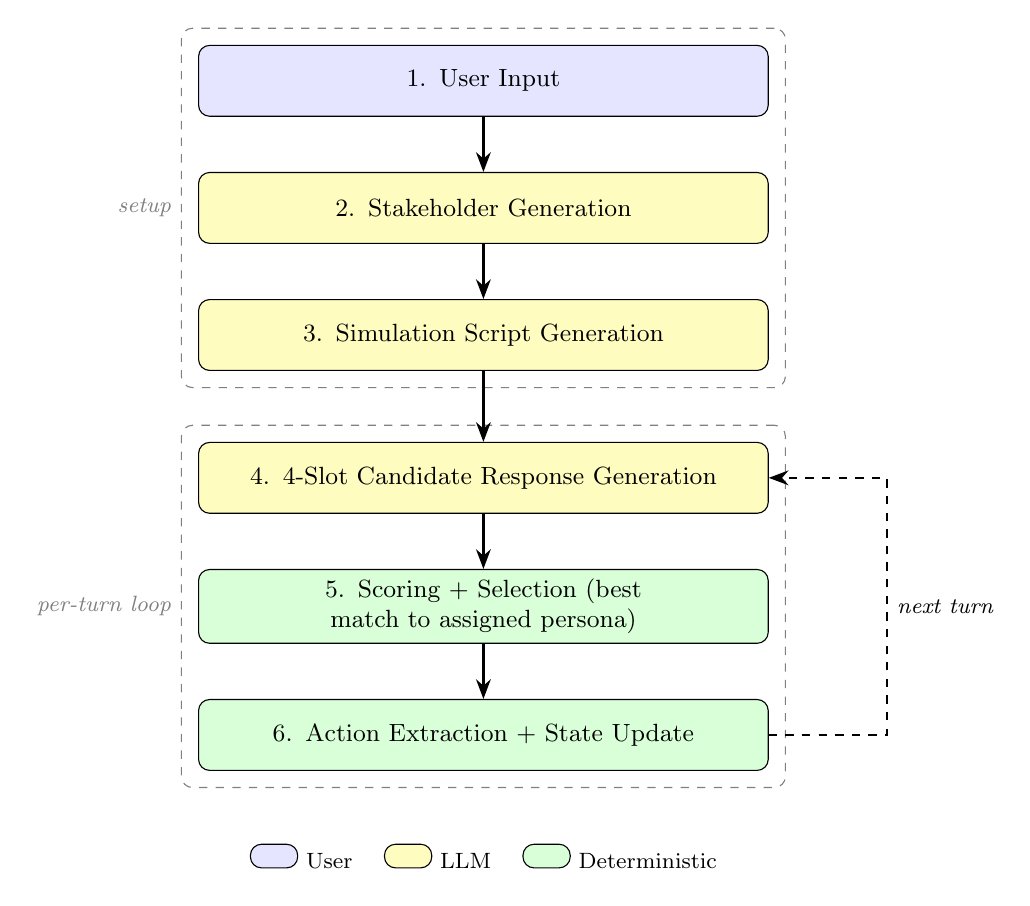
\begin{tikzpicture}[
    node distance=0.7cm,
    every node/.style={font=\small},
    inputbox/.style={rectangle, draw, rounded corners, fill=blue!10, text width=7cm, minimum height=0.9cm, align=center},
    llmbox/.style={rectangle, draw, rounded corners, fill=yellow!25, text width=7cm, minimum height=0.9cm, align=center},
    detbox/.style={rectangle, draw, rounded corners, fill=green!15, text width=7cm, minimum height=0.9cm, align=center},
    arr/.style={-{Stealth[length=2.5mm]}, thick},
    looparr/.style={-{Stealth[length=2.5mm]}, thick, dashed}
]
% Setup phase
\node[inputbox] (input) {1. User Input};
\node[llmbox, below=of input] (gen) {2. Stakeholder Generation};
\node[llmbox, below=of gen] (script) {3. Simulation Script Generation};

% Per-turn loop
\node[llmbox, below=0.9cm of script] (cand) {4. 4-Slot Candidate Response Generation};
\node[detbox, below=of cand] (score) {5. Scoring + Selection (best match to assigned persona)};
\node[detbox, below=of score] (action) {6. Action Extraction + State Update};

% Arrows
\draw[arr] (input) -- (gen);
\draw[arr] (gen) -- (script);
\draw[arr] (script) -- (cand);
\draw[arr] (cand) -- (score);
\draw[arr] (score) -- (action);

% Per-turn loop back
\draw[looparr] (action.east) -- ++(1.5,0) |- node[right, pos=0.25, font=\footnotesize\itshape] {next turn} (cand.east);

% Grouping labels
\begin{scope}[on background layer]
    \node[draw=gray, dashed, rounded corners, inner sep=6pt, fit=(input)(gen)(script), label={[font=\footnotesize\itshape, text=gray]left:setup}] {};
    \node[draw=gray, dashed, rounded corners, inner sep=6pt, fit=(cand)(score)(action), label={[font=\footnotesize\itshape, text=gray]left:per-turn loop}] {};
\end{scope}

% Legend
\node[below=0.8cm of action, font=\footnotesize, anchor=north] (legend) {
    \tikz{\node[fill=blue!10, draw, rounded corners, minimum width=0.6cm, minimum height=0.3cm] {};} User \quad
    \tikz{\node[fill=yellow!25, draw, rounded corners, minimum width=0.6cm, minimum height=0.3cm] {};} LLM \quad
    \tikz{\node[fill=green!15, draw, rounded corners, minimum width=0.6cm, minimum height=0.3cm] {};} Deterministic
};
\end{tikzpicture}
\caption{Simulation engine workflow. The setup phase (steps 1--3) runs once per simulation. The per-turn loop (steps 4--6) repeats for each stakeholder's turn.}
\label{fig:architecture}
\end{figure}

The workflow consists of a \textbf{setup phase} (steps 1--3) that runs once, followed by a \textbf{per-turn loop} (steps 4--6) that repeats for every stakeholder turn:

\begin{enumerate}[leftmargin=*, itemsep=2pt]
    \item \textbf{User Input} --- the user provides a scenario and selects guided or exploratory mode.
    \item \textbf{Stakeholder Generation} --- the LLM generates stakeholders with OCEAN profiles, incentives, and concerns (Section~3.2).
    \item \textbf{Simulation Script Generation} --- stakeholders and stage structure are assembled into a structured configuration (Section~3.2).
    \item \textbf{Candidate Response Generation} --- four candidate responses are generated per turn, each in a different rhetorical style (Section~3.3).
    \item \textbf{Behavioural Scoring + Selection} --- each candidate is scored against the stakeholder's assigned persona; the best match is selected (Section~3.4).
    \item \textbf{Action Extraction + State Update} --- structured actions are extracted and simulation state is updated (Section~3.5).
\end{enumerate}

Steps 4--6 repeat for each stakeholder in each stage until the deliberation is complete. The full pseudocode is provided in Algorithm~\ref{alg:main_loop} in Appendix~\ref{app:main_loop}. The following sections describe each step in detail.


Fig.~\ref{fig:layers} shows how the engine's components are organised into layers, and which sub-components belong to each. The following sections (3.2--3.5) describe each layer in detail.

\begin{figure}[ht]
\centering
\resizebox{\textwidth}{!}{%
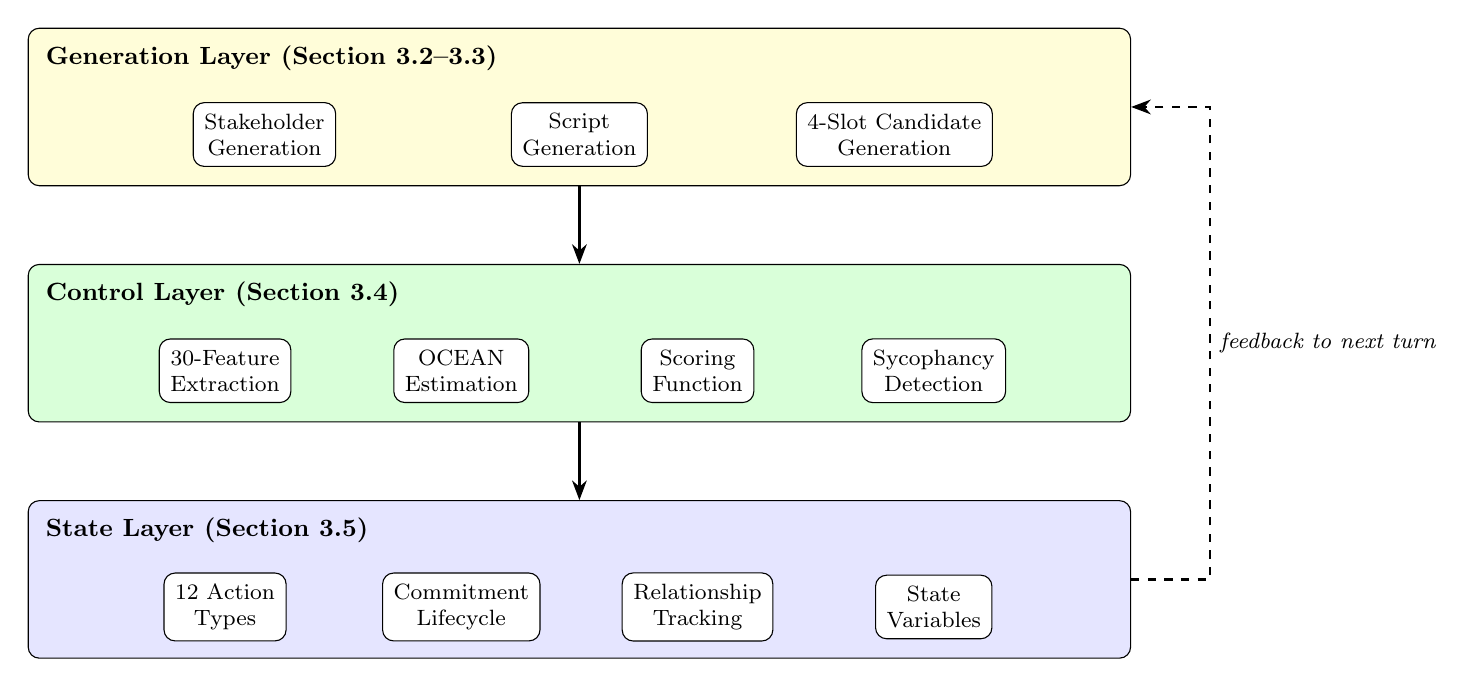
\begin{tikzpicture}[
    every node/.style={font=\small},
    layerbox/.style={rectangle, draw, rounded corners, minimum width=14cm, minimum height=2cm, align=center},
    subbox/.style={rectangle, draw, rounded corners, fill=white, minimum height=0.7cm, align=center, font=\footnotesize, inner sep=4pt},
    arr/.style={-{Stealth[length=2.5mm]}, thick}
]

% Generation Layer
\node[layerbox, fill=yellow!15] (gen) at (0, 0) {};
\node[anchor=north west, font=\small\bfseries] at ([shift={(3pt,-3pt)}]gen.north west) {Generation Layer (Section 3.2--3.3)};
\node[subbox] (g1) at (-4, -0.35) {Stakeholder\\Generation};
\node[subbox] (g2) at (0, -0.35) {Script\\Generation};
\node[subbox] (g3) at (4, -0.35) {4-Slot Candidate\\Generation};

% Control Layer
\node[layerbox, fill=green!15] (ctrl) at (0, -3) {};
\node[anchor=north west, font=\small\bfseries] at ([shift={(3pt,-3pt)}]ctrl.north west) {Control Layer (Section 3.4)};
\node[subbox] (c1) at (-4.5, -3.35) {30-Feature\\Extraction};
\node[subbox] (c2) at (-1.5, -3.35) {OCEAN\\Estimation};
\node[subbox] (c3) at (1.5, -3.35) {Scoring\\Function};
\node[subbox] (c4) at (4.5, -3.35) {Sycophancy\\Detection};

% State Layer
\node[layerbox, fill=blue!10] (state) at (0, -6) {};
\node[anchor=north west, font=\small\bfseries] at ([shift={(3pt,-3pt)}]state.north west) {State Layer (Section 3.5)};
\node[subbox] (s1) at (-4.5, -6.35) {12 Action\\Types};
\node[subbox] (s2) at (-1.5, -6.35) {Commitment\\Lifecycle};
\node[subbox] (s3) at (1.5, -6.35) {Relationship\\Tracking};
\node[subbox] (s4) at (4.5, -6.35) {State\\Variables};

% Arrows between layers
\draw[arr] (gen.south) -- (ctrl.north);
\draw[arr] (ctrl.south) -- (state.north);
\draw[arr, dashed] (state.east) -- ++(1,0) |- node[right, pos=0.25, font=\footnotesize\itshape] {feedback to next turn} (gen.east);

\end{tikzpicture}%
}
\caption{Layer architecture of the simulation engine. The Generation Layer produces candidate responses (LLM). The Control Layer scores and selects responses using rule-based scoring. The State Layer extracts actions (keyword matching with LLM fallback) and maintains persistent state. The dashed arrow indicates that state feeds back into the next turn's generation context.}
\label{fig:layers}
\end{figure}


\section{Stakeholder and Script Generation}

This section covers steps 2 and 3 of the workflow: how the engine generates stakeholders and assembles the simulation script.

\subsection{Stakeholder Generation}

Given a scenario, the LLM generates a cast of stakeholders. Each stakeholder is defined by:

\begin{itemize}[leftmargin=*, itemsep=1pt]
    \item \textbf{Role and name} --- e.g., ``John Doe, Financial Regulator''
    \item \textbf{OCEAN personality profile} --- five continuous values between 0.0 and 1.0
    \item \textbf{Incentives} --- what this stakeholder wants to achieve
    \item \textbf{Concerns} --- what this stakeholder wants to avoid
    \item \textbf{Strategic disposition} --- one of four orientations: \texttt{cooperative}, \texttt{neutral}, \texttt{competitive}, or \texttt{adversarial}, with a strength value ($0.0$--$1.0$)
\end{itemize}

The strategic disposition was introduced because, without it, all stakeholders default to neutral-cooperative behaviour regardless of their role. A union leader and a corporate executive should not negotiate in the same tone. The disposition affects three things: (1) the tone of the system prompt used for generation, (2) which action types the stakeholder is biased toward, and (3) how aggressively sycophancy is penalised for that stakeholder --- an adversarial stakeholder agreeing with everyone is more suspicious than a cooperative one doing the same.

\subsection{Simulation Script}

The generated stakeholders are assembled into a simulation script --- a structured JSON configuration that defines:

\begin{itemize}[leftmargin=*, itemsep=1pt]
    \item The scenario context and background
    \item The full stakeholder roster with all attributes above
    \item The stage sequence (typically OPENING $\to$ TENSION $\to$ NEGOTIATION $\to$ CLOSING)
    \item For guided mode: the expected outcome at each stage
\end{itemize}

The four-stage structure reflects how real deliberations tend to progress: stakeholders first establish their positions (OPENING), then encounter disagreements (TENSION), attempt to find compromise (NEGOTIATION), and finally reach or fail to reach resolution (CLOSING). This structure is important because the engine applies different scoring weights at each stage, as described in the next section.


\section{Candidate Response Generation}

This section covers step 4: how the engine generates diverse candidate responses for each stakeholder's turn.

\subsection{Why Four Candidates}

A single LLM generation per turn tends to produce the same cooperative, agreeable style regardless of the stakeholder's assigned personality. This is the sycophancy problem described in Chapter~1. Generating four candidates with different rhetorical styles gives the scoring system something to choose from --- if one candidate is sycophantic, another might express the stakeholder's personality more faithfully.

\subsection{The Four Rhetorical Styles}

The four styles and their typical action preferences are shown in Table~\ref{tab:slots}.

\begin{table}[t]
\centering
\caption{4-Slot Candidate Response Styles}
\label{tab:slots}
\begin{tabular}{p{2cm}p{4cm}p{4cm}}
\toprule
Style & Behaviour & Typical Actions \\
\midrule
Integrator & Seeks common ground, builds on others' points & \texttt{assign\_owner}, \texttt{commit\_resource}, \texttt{publish\_update} \\
Planner & Proposes structured plans and timelines & \texttt{set\_deadline}, \texttt{narrow\_scope}, \texttt{pilot} \\
Challenger & Questions assumptions, pushes back & \texttt{preserve\_autonomy}, \texttt{request\_evidence}, \texttt{escalate} \\
Skeptic & Expresses doubt, requests evidence & \texttt{audit\_compliance}, \texttt{defer\_decision}, \texttt{request\_evidence} \\
\bottomrule
\end{tabular}
\end{table}

These four styles were chosen to cover the range of rhetorical strategies observed in real multi-party deliberation. Two styles lean cooperative (integrator, planner) and two lean confrontational (challenger, skeptic), ensuring that the candidate pool always contains at least some diversity in tone. This is particularly important for stakeholders with low Agreeableness or adversarial dispositions, who need confrontational candidates to choose from.


\section{Behavioural Scoring and Selection}

This section covers step 5: how the engine scores each candidate response against the stakeholder's assigned personality and selects the best match.

\subsection{30-Feature Behavioural Extraction}

Each candidate response is analysed using 30 linguistic features, organised by their primary OCEAN trait association. Table~\ref{tab:features} shows a representative subset; the complete specification is in Appendix~\ref{app:features}.

\begin{table}[t]
\centering
\caption{Representative Behavioural Features (subset of 30). The full specification is in Appendix~\ref{app:features}.}
\label{tab:features}
\small
\begin{tabular}{llll}
\toprule
Feature & OCEAN Trait & Detection Method & Example Cues \\
\midrule
\texttt{idea\_count}            & Openness (O)        & Keyword matching   & ``what if'', ``we could'' \\
\texttt{planning\_count}        & Conscientiousness (C) & Keyword matching & ``plan'', ``timeline'', ``step'' \\
\texttt{avg\_words\_per\_turn}  & Extraversion (E)    & Word count per turn & (numerical, no keywords) \\
\texttt{disagreement\_count}    & Agreeableness (A)   & Keyword matching   & ``disagree'', ``however'' \\
\texttt{hedge\_count}           & Neuroticism (N)     & Keyword matching   & ``maybe'', ``perhaps'' \\
\bottomrule
\end{tabular}
\end{table}

These features were chosen because each maps to a specific OCEAN trait through established psycholinguistic research~\cite{mairesse2007personality}. For example, word count is a reliable indicator of Extraversion, and hedging language correlates with Neuroticism. The \texttt{acknowledgment\_count} feature specifically targets sycophancy --- excessive agreement that does not match the stakeholder's assigned Agreeableness level.

\subsection{OCEAN Estimation with Dynamic Calibration}

Raw feature counts are converted to OCEAN trait estimates using dynamic calibration. Absolute feature counts alone are not meaningful without context. For example, a \texttt{planning\_count} of 3 signals high Conscientiousness in a casual conversation, but is commonly used in a project management scenario where everyone uses planning language. To account for this, the engine does the following:

\begin{enumerate}[leftmargin=*, itemsep=1pt]
    \item Compute the average feature values across all other stakeholders in the conversation (the \textit{conversation baseline}).
    \item Compare each stakeholder's feature values against this baseline to determine whether they are above or below average.
    \item Multiply the difference by a calibration coefficient ($\lambda$) and add it to a centre point of 0.50 to produce the trait estimate.
\end{enumerate}

The formal pseudocode is provided in Algorithm~\ref{alg:ocean} in Appendix~\ref{app:main_loop}.

The calibration coefficients $\lambda_t$ control how sensitive each trait estimate is to deviations from the baseline (Table~\ref{tab:lambda}).

\begin{table}[t]
\centering
\caption{OCEAN Calibration Coefficients}
\label{tab:lambda}
\begin{tabular}{lcp{6cm}}
\toprule
Trait & $\lambda$ & Justification \\
\midrule
Openness (O) & 0.55 & Moderate signal from idea count and hypothetical language \\
Conscientiousness (C) & 0.55 & Moderate signal, but planning language is common in deliberation contexts \\
Extraversion (E) & 0.65 & Strong signal from word count, question frequency, and turn initiation --- these are the most reliable verbal indicators \\
Agreeableness (A) & 0.50 & Moderate signal; disagreement keywords can be ambiguous \\
Neuroticism (N) & 0.50 & Weakest signal due to RLHF suppression of anxiety expressions \\
\bottomrule
\end{tabular}
\end{table}

The state ledger maintains a rolling estimate of each stakeholder's trait expression using exponential smoothing ($\alpha = 0.6$ for the current turn, $0.4$ for history). This prevents a single unusual turn from triggering overcorrection.

All numerical values in this section --- the $\lambda$ coefficients, the smoothing factor $\alpha$, and the 0.50 centre point --- were determined through a series of preliminary calibration experiments conducted prior to the main benchmark. The process and results of these experiments are described in Section~4.1.

\subsection{Scoring Function}

Each candidate response is scored using four components, with weights that vary depending on which stage of the deliberation the simulation is in --- OPENING, TENSION, NEGOTIATION, or CLOSING (Algorithm~\ref{alg:scoring} in Appendix~\ref{app:main_loop}):

\begin{enumerate}[leftmargin=*, itemsep=2pt]
    \item \textbf{Persona score.} The engine estimates what OCEAN traits the response expresses, then computes the average difference from the stakeholder's assigned profile. A smaller difference means a higher score. For example, if a stakeholder is assigned Agreeableness = 0.3 but the response expresses Agreeableness = 0.7, the persona score drops.
    \item \textbf{Sycophancy penalty.} The response is checked for excessive agreement. A response full of ``great point'' and ``I agree'' receives a higher sycophancy score, which lowers the overall score. The detection uses four layers that amplify the risk based on context: (1) base risk from agreement keywords, (2) higher penalty if the scenario has high conflict --- agreement in a hostile negotiation is more suspicious than in a cooperative one, (3) higher penalty if the stakeholder has an adversarial or competitive disposition, and (4) higher penalty if the stakeholder has low assigned Agreeableness, since such a stakeholder should not be agreeing easily. The formal pseudocode is in Algorithm~\ref{alg:sycophancy} in Appendix~\ref{app:main_loop}.
    \item \textbf{Social alignment.} The response is checked for trait-appropriate social behaviour. For example, a high-Extraversion stakeholder should speak more and ask more questions; a low-Agreeableness stakeholder should push back rather than comply.
    \item \textbf{Envelope penalty.} If any trait deviates more than 0.15 from the assigned value, a squared penalty is applied. Small deviations are handled by the persona score, but large deviations (e.g., 0.30 away from assigned) are penalised much more heavily through this super-linear term.
\end{enumerate}

These four components are combined into a weighted sum, where the weights change depending on the current stage (Table~\ref{tab:phase_weights}). The rationale is that different stages have different failure modes:

\begin{table}[t]
\centering
\caption{Stage-Specific Weight Modifiers}
\label{tab:phase_weights}
\begin{tabular}{lccccl}
\toprule
Stage & Persona & Syc. & Social & Env. & Rationale \\
\midrule
OPENING & 1.2$\times$ & 0.8$\times$ & 1.0$\times$ & 1.0$\times$ & Establishing positions; persona matters most \\
TENSION & 1.0$\times$ & 1.8$\times$ & 1.4$\times$ & 1.0$\times$ & Conflict stage; agreement is most suspicious here \\
NEGOTIATION & 1.0$\times$ & 1.0$\times$ & 1.0$\times$ & 1.3$\times$ & Compromise stage; prevent extreme trait violations \\
CLOSING & 1.3$\times$ & 1.0$\times$ & 1.0$\times$ & 1.4$\times$ & ``Summarize and agree'' tendency; reinforce persona \\
\bottomrule
\end{tabular}
\end{table}

All weight values were determined through the preliminary calibration experiments described in Section~4.1.


\section{Action Extraction and State Management}

This section covers step 6: how the engine extracts structured actions from dialogue and tracks simulation state across turns.

\subsection{12 Action Types}

Dialogue alone does not capture the decisions stakeholders make during deliberation. When a regulator says ``we should audit the compliance records before proceeding,'' that is not just a statement --- it is an action (\texttt{audit\_compliance}) that should reduce uncertainty in the simulation state. The engine defines 12 action types organised in 6 families (Table~\ref{tab:actions}), each with a specific effect on the simulation's state variables.

The 6 families are informed by speech act theory~\cite{searle1975taxonomy} and deliberation dialogue frameworks~\cite{walton1995commitment}. Searle's taxonomy classifies speech acts into directives (requesting action), commissives (committing to future action), and declarations (changing the state of affairs) --- which map directly to action families like Evidence (directives: requesting data), Resourcing (commissives: committing resources), and Governance (declarations: escalating or auditing). Walton and Krabbe's deliberation model defines moves such as propose, revise, and recommend, which correspond to Scope (narrowing or piloting proposals) and Timing (setting deadlines or deferring). The 12 specific action types within these families were refined from patterns observed across the 20 benchmark scenarios during preliminary experiments (Section~4.1).

\begin{table}[t]
\centering
\caption{12 Structured Action Types and Their Effects}
\label{tab:actions}
\begin{tabular}{llcl}
\toprule
Family & Action Type & State Effect & Why This Effect \\
\midrule
Ownership   & \texttt{assign\_owner}      & trust +0.04 & Taking responsibility builds trust \\
Evidence    & \texttt{request\_evidence}   & uncertainty $-$0.04 & Asking for data reduces ambiguity \\
Comms       & \texttt{publish\_update}     & alignment +0.04 & Transparency increases alignment \\
\multirow{2}{*}{Scope}
            & \texttt{narrow\_scope}       & uncertainty $-$0.04 & Focusing reduces unknowns \\
            & \texttt{pilot}               & risk $-$0.08 & Testing before full rollout reduces risk \\
\multirow{2}{*}{Resourcing}
            & \texttt{commit\_resource}    & confidence +0.08 & Backing words with resources signals commitment \\
            & \texttt{allocate\_budget}    & confidence +0.08 & Same as above \\
\multirow{2}{*}{Timing}
            & \texttt{set\_deadline}       & uncertainty $-$0.04 & Deadlines create clarity \\
            & \texttt{defer\_decision}     & tension $-$0.04 & Delaying can reduce immediate pressure \\
\multirow{3}{*}{Governance}
            & \texttt{preserve\_autonomy}  & tension +0.08 & Resisting control increases friction \\
            & \texttt{escalate}            & tension +0.12 & Escalating raises the stakes \\
            & \texttt{audit\_compliance}   & uncertainty $-$0.08 & Formal review provides clarity \\
\bottomrule
\end{tabular}
\end{table}

The delta values (+0.04, +0.08, +0.12) were chosen to create meaningful but not overwhelming state changes. Single actions produce small shifts; only accumulated actions over multiple turns produce large state movements. The larger deltas (0.08, 0.12) are reserved for actions with stronger real-world consequences --- committing resources or escalating a dispute has more impact than publishing an update. These values were calibrated through the preliminary experiments described in Section~4.1.

\subsection{Action Extraction Pipeline}

Actions are extracted from the selected response using a three-stage pipeline (Algorithm~\ref{alg:action} in Appendix~\ref{app:main_loop}):

\begin{enumerate}[leftmargin=*, itemsep=2pt]
    \item \textbf{Policy plan check.} If the stakeholder's policy plan specifies a planned action, the engine tries to match it first. This has the highest priority.
    \item \textbf{Keyword matching (deterministic).} The engine scans the response for action-bearing keywords and matches them to one of the 12 action types. It also detects the strength of the action (strong/medium/weak) from modal verbs like ``must'' vs ``could''. If the confidence exceeds 0.62, the action is accepted.
    \item \textbf{LLM fallback.} If keywords did not match but the response appears to contain an action, the LLM is asked to classify the action type directly. This uses temperature = 0 to keep the extraction deterministic.
\end{enumerate}

The confidence threshold of 0.62 was calibrated in Section~4.1 to balance precision and recall. During the OPENING stage, actions are detected but not executed (shadow mode), since stakeholders are still establishing positions and should not be committing to actions yet.

\subsection{Commitment Lifecycle}

Stakeholders frequently make commitments during deliberation (``I will prepare the draft by Friday'') but may fail to follow through or contradict themselves later. The engine tracks all commitments through a four-stage lifecycle (Algorithm~\ref{alg:commitment} in Appendix~\ref{app:main_loop}):

\begin{enumerate}[leftmargin=*, itemsep=2pt]
    \item \textbf{Extraction.} The LLM identifies any new commitments in the stakeholder's response and adds them to the ledger with status ``open''.
    \item \textbf{Fulfillment detection.} Each open commitment is checked against the current response to see if it has been fulfilled.
    \item \textbf{Stage-based resolution.} Commitments tied to the current stage are resolved when that stage ends.
    \item \textbf{Staleness.} Commitments older than 8 turns are marked ``stale'', preventing the ledger from accumulating outdated positions that no longer reflect the discussion.
\end{enumerate}

After processing, the engine injects ``Your prior positions: [list of open commitments]'' into the next generation prompt.

A critical design insight emerged from early experiments: explicitly instructing stakeholders to ``stay consistent unless explicitly revising'' caused behavioural diversity to collapse to 0.45, as stakeholders rigidly repeated their initial positions. The successful approach is \textit{informational} --- simply listing ``Your prior positions: [...]'' without any directive, and letting the LLM decide how to use that information. In the main benchmark, contradiction rates were 0.000 under both engine and naive conditions, so the commitment lifecycle's primary contribution is in improving fulfillment tracking and state traceability rather than contradiction prevention alone.

\subsection{Relationship and State Tracking}

Beyond commitments, the engine tracks pairwise relationships between stakeholders (trust, alignment) and global state variables (tension, uncertainty, confidence, risk). These are updated after each action and fed back into the generation context for the next turn, creating a feedback loop where past actions influence future behaviour.


% ══════════════════════════════════════════════════════════════════════
% CHAPTER 4: EXPERIMENTAL SETUP
% ══════════════════════════════════════════════════════════════════════
\chapter{Evaluation Methodology}

This chapter details the experimental design used to validate the simulation engine. Section~4.1 describes the preliminary calibration experiments that determined the engine's hyperparameters. Sections~4.2 onwards describe the main 4,080-run benchmark.


\section{Preliminary Calibration Experiments}

Before the main benchmark, a series of preliminary experiments were conducted to calibrate the engine's hyperparameters. Each experiment changed one or two variables while holding others fixed, and the results determined the final parameter values used in the main benchmark. Table~\ref{tab:calibration} summarises these experiments and their outcomes.

\begin{table}[t]
\centering
\caption{Preliminary Calibration Experiments}
\label{tab:calibration}
\small
\begin{tabular}{clp{4.5cm}p{4.5cm}}
\toprule
Exp & Focus & What Was Tested & Outcome \\
\midrule
1 & Drift control & Added E/A/N drift regularisation penalties & Drift reduced from 0.190 to 0.163 \\
2 & E/O stability & E stability penalty, relationship sentiment refinement & O error $-$9\%, E error $-$8\% \\
3 & Ablation & Removed individual components one at a time & Trait poles most critical (+0.015 drift if removed) \\
4 & Domain test & Tested engine on non-policy scenarios & Engine generalises: drift 0.176 (naive) $\to$ 0.159 (engine) \\
5 & Action layer & Tested action-aware scoring (v0.0--v0.6) & Action-aware scoring was harmful; dialogue-only scoring retained \\
6 & Two-track & Separated guided vs exploratory modes & Guided drift 0.159, exploratory drift 0.181 \\
\midrule
A & Commitment & Tested directive vs informational prompt injection & Directive collapsed diversity to 0.45; informational achieved 0 contradictions + diversity 0.619 \\
B & Scaling & Tested 2/3/5-actor configurations & Drift increase minimal (+0.009 from 2 to 5 actors) \\
\bottomrule
\end{tabular}
\end{table}

Key calibration decisions that emerged from these experiments:

\begin{itemize}[leftmargin=*, itemsep=2pt]
    \item \textbf{OCEAN calibration coefficients} ($\lambda_O = 0.55$, $\lambda_C = 0.55$, $\lambda_E = 0.65$, $\lambda_A = 0.50$, $\lambda_N = 0.50$). Extraversion received the highest coefficient (0.65) because verbal features like word count and question frequency showed the strongest signal-to-noise ratio in Experiments 1--2. Neuroticism received the lowest (0.50) because RLHF suppression made its signal inherently weak.

    \item \textbf{Rolling estimate smoothing} ($\alpha = 0.6$). Values below 0.5 made trait estimates too slow to respond to genuine behavioural shifts; values above 0.7 caused overcorrection from single-turn anomalies. The value 0.6 was selected as the best balance in Experiment 2.

    \item \textbf{Stage-specific sycophancy weight} (TENSION: 1.8$\times$). Experiments 1--2 showed that sycophantic agreement was most damaging during the conflict stage, where stakeholders should be disagreeing. The 1.8$\times$ multiplier was the minimum value that consistently penalised false agreement in high-conflict scenarios without suppressing legitimate agreement in low-conflict ones.

    \item \textbf{Envelope penalty threshold} ($\tau = 0.15$). Deviations below 0.15 were within normal variation; deviations above 0.15 consistently indicated persona boundary violations in Experiment 3's ablation analysis.

    \item \textbf{Action confidence threshold} ($\sigma = 0.62$). Lower values (e.g., 0.45) produced too many false-positive action extractions; higher values (e.g., 0.75) missed legitimate actions. The value 0.62 balanced precision and recall in Experiment 5.

    \item \textbf{Commitment staleness} ($\tau = 8$ turns). Commitments older than 8 turns (roughly two full rounds of deliberation) were rarely referenced again. This was observed in Arm A experiments.

    \item \textbf{Soft prompt design} (``Your prior positions: [list]''). Arm A showed that directive prompts (``stay consistent unless explicitly revising'') collapsed diversity to 0.45, while informational prompts (just listing prior positions without instructions) maintained diversity at 0.619 with zero contradictions.
\end{itemize}


\section{Scenarios}

The benchmark comprises 20 real-world policy and corporate scenarios drawn from six domains (Table~\ref{tab:scenarios}). Each scenario is instantiated at three actor scales (3, 5, and 10 agents), yielding 60 unique simulation scripts.

\begin{table}[t]
\centering
\caption{20 Benchmark Scenarios by Domain}
\label{tab:scenarios}
\begin{tabular}{p{3.5cm}cp{10cm}}
\toprule
Domain & $n$ & Examples \\
\midrule
Policy / Regulatory    & 7 & EU GDPR, NYC Congestion Pricing, CA AB5 Gig Worker Law, Australia Robodebt \\
Corporate Crisis       & 4 & FTX Collapse, Boeing 737 MAX, WeWork IPO, Theranos \\
Labor / Workplace      & 3 & Starbucks Unionization, Amazon Labor, Zoom RTO \\
Ethics / Technology    & 2 & UK Post Office Horizon, Microsoft-Activision Merger \\
Financial / Consumer   & 2 & Netflix Password Crackdown, Peloton Demand Cliff \\
Public Health / Infra. & 2 & Flint Water Crisis, Fukushima Nuclear Restart \\
\bottomrule
\end{tabular}
\end{table}

All 20 scenarios are based on real-world events. In a production deployment, a simulation engine would use RAG (Retrieval-Augmented Generation) or live search to supply factual context about the scenario. Since this engine does not yet implement RAG (see Chapter~7), scenarios were chosen from events that LLMs have already been trained on, so that the model's pre-training knowledge serves as a substitute for external data retrieval. This ensures that stakeholders have sufficient factual grounding to deliberate realistically, while isolating behavioural fidelity as the variable being tested. This design choice is acknowledged as a limitation: LLMs may produce responses informed by factual recall rather than genuine persona-driven reasoning.

Each scenario is automatically assigned a \textit{structural profile} based on two factors: a conflict ratio (computed from keyword overlap between stakeholders' incentives and concerns) and a pressure level (derived from the number of actors and stages). The conflict ratio classifies scenarios as adversarial, fragmented, or collaborative, which in turn modulates the engine's sycophancy detection sensitivity, initial tension levels, and trust decay rates (see Section~3.4).


\section{Experimental Conditions}

Two experimental conditions are compared:

\textbf{Engine Structural (\engine):} The full simulation engine (Fig.~\ref{fig:architecture}) with all components active. Each turn generates 4 candidate responses, scores them deterministically against the stakeholder's assigned persona, and selects the best match.

\textbf{Naive Prompting (\naive):} Each stakeholder receives only a persona prompt (OCEAN personality priors, role description, incentives, and concerns) and generates a single response per turn without candidate pooling, scoring, or any engine-level control. This represents the standard approach to LLM-based role-playing. An example of the naive prompt is provided in Appendix~\ref{app:prompts}.

The main benchmark compares the full engine against naive prompting, rather than testing each layer (Fig.~\ref{fig:layers}) separately. The effect of individual layers was already tested during the preliminary experiments (Section~4.1). The main benchmark focuses on whether the complete engine as a whole improves over naive prompting.



\section{Scale}

Table~\ref{tab:scale} summarizes the benchmark scale.

\begin{table}[t]
\centering
\caption{Benchmark Scale}
\label{tab:scale}
\begin{tabular}{lr}
\toprule
Parameter & Value \\
\midrule
Scenario configurations (20 scenarios $\times$ 3 actor scales) & 60 \\
Conditions                        & 2 \\
Repetitions per (configuration, condition) & $\sim$34 \\
\textbf{Total runs}               & \textbf{4,080} \\
  \quad Engine runs               & 2,056 \\
  \quad Naive runs                & 2,024 \\
Average turns per run             & 11 \\
LLM calls per run (engine)       & $\sim$88 \\
LLM calls per run (naive)        & $\sim$22 \\
Total LLM calls (estimated)      & $\sim$120,000+ \\
Approximate total runtime         & $\sim$50 hours \\
Generation model                  & DeepSeek V3 \\
\bottomrule
\end{tabular}
\end{table}

Each (configuration, condition) pair was repeated approximately 34 times because LLM outputs vary between runs even with the same input. Repeating ensures that the results reflect stable patterns rather than single-run variance, and provides enough data for statistical significance testing.


\section{Metrics}
\label{sec:metrics}

The evaluation framework comprises three groups of metrics: \textit{deterministic primary fidelity metrics} that directly measure persona maintenance, a \textit{deterministic outcome metric} derived from ground-truth scenario comparisons, and \textit{secondary diagnostics} that capture how the engine changes conversation dynamics and decision-making behaviour.

\subsection{Primary Metrics}

\textbf{Persona Drift MAE.} The primary metric is the Mean Absolute Error between the inferred OCEAN trait expression and the assigned personality prior, averaged across all five traits and all turns within a run:

\begin{equation}
    \text{Drift} = \frac{1}{5} \sum_{t \in \text{OCEAN}} \left| \hat{\theta}_t - \pi_t \right|
    \label{eq:drift}
\end{equation}

\noindent where $\hat{\theta}_t$ is the estimated trait value from the 30-feature extraction pipeline and $\pi_t$ is the assigned prior. Lower values indicate better persona maintenance.

\textit{Justification:} MAE was chosen over MSE because persona drift in practice involves small, consistent deviations rather than occasional large spikes; MAE provides a more interpretable measure of typical per-trait error magnitude. The choice of OCEAN trait estimation through behavioural feature extraction (rather than LLM self-assessment) follows from Stureborg~\etal's finding that LLM-based evaluators are inconsistent and biased~\cite{stureborg2024inconsistent}---a deterministic pipeline ensures reproducibility.

\textbf{Envelope Violations.} The count of OCEAN traits exceeding a threshold $\tau = 0.15$ from the assigned prior per run:

\begin{equation}
    \text{Violations} = \sum_{t \in \text{OCEAN}} \mathbb{1}\!\left[|\hat{\theta}_t - \pi_t| > \tau\right]
    \label{eq:envelope}
\end{equation}

\textit{Justification:} While Drift MAE captures the average deviation, Envelope Violations capture the \textit{frequency} of significant personality boundary breaches.


\subsection{Outcome Fidelity}

Because all 20 scenarios are based on real-world events with documented outcomes, the simulation results can be compared against what actually happened. Outcome fidelity measures this similarity across six dimensions: (1) whether the simulation reached a similar resolution, (2) whether stakeholders ended up in similar positions, (3) whether the dynamics followed a similar pattern, (4) whether key turning points occurred, (5) whether the world-state changes matched, and (6) whether the distribution of actions was realistic. The score ranges from 0.0 (no similarity) to 1.0 (exact match). This comparison is computed deterministically against a structured ground-truth record for each scenario using these six rubric components.

Unlike the primary fidelity metrics which are compared using paired $t$-tests at the run level, outcome fidelity is aggregated at the scenario-condition level and analysed with Welch's $t$-test.


\subsection{Secondary Diagnostics}

Table~\ref{tab:metrics_overview} provides an overview of all metrics by category.

\begin{table}[t]
\centering
\caption{Metrics Overview by Category}
\label{tab:metrics_overview}
\small
\begin{tabular}{llll}
\toprule
Category & Metric & Type & Higher is \\
\midrule
\multirow{2}{*}{Persona Fidelity}
    & Drift MAE & Primary & Worse \\
    & Envelope Violations & Primary & Worse \\
\midrule
Outcome & Outcome Fidelity & Outcome & Better \\
\midrule
\multirow{2}{*}{Consistency}
    & Contradiction Rate & Secondary & Worse \\
    & Fulfillment Rate & Secondary & Better \\
\midrule
\multirow{5}{*}{Dialogue}
    & Convergence & Secondary & Worse \\
    & Semantic Identity Consistency & Secondary & Better \\
    & Dialogue Coherence & Secondary & Better \\
    & Topic Drift Rate & Secondary & Worse \\
    & Repetition Rate & Secondary & Worse \\
\midrule
\multirow{4}{*}{Behavioural}
    & Acknowledgment Count & Secondary & Worse \\
    & Disagreement Count & Secondary & Better \\
    & Idea Count & Secondary & Better \\
    & Self-Doubt Count & Secondary & Better \\
\midrule
\multirow{3}{*}{Action}
    & Diversity & Secondary & Better \\
    & Action-Plan Alignment & Secondary & Better \\
    & Action Validity Rate & Secondary & Better \\
\bottomrule
\end{tabular}
\end{table}

\textbf{Commitment Contradiction Rate.} The proportion of turns that contradict a prior commitment by the same stakeholder. A value of 0.000 indicates perfect consistency.

\textbf{Commitment Fulfillment Rate.} The proportion of stated commitments that are subsequently fulfilled.

\textbf{Convergence.} Pairwise semantic similarity across stakeholders' utterances within a turn, computed using sentence-transformer embeddings. Values approaching 1.0 indicate homogenised viewpoints:

\begin{equation}
    \text{Convergence} = \frac{2}{n(n-1)} \sum_{i < j} \text{cos}(\mathbf{e}_i, \mathbf{e}_j)
    \label{eq:convergence}
\end{equation}

\textbf{Diversity.} The ratio of unique action types to total actions per run. Higher values indicate more varied decision-making:

\begin{equation}
    \text{Diversity} = \frac{|\text{unique action types}|}{|\text{total actions}|}
    \label{eq:diversity}
\end{equation}

\textbf{Acknowledgment Count.} Sycophantic agreement expressions per turn.

\textbf{Disagreement Count.} Explicit disagreement expressions per turn.

\textbf{Idea Count.} Novel proposals per turn, measuring informational value.

\textbf{Self-Doubt Count.} Expressions of self-doubt per turn. This metric directly probes the RLHF ceiling for Neuroticism.

\textbf{Action-Plan Alignment.} The proportion of executed actions consistent with the stakeholder's stated plan.

\textbf{Action Validity Rate.} The proportion of extracted actions that are structurally valid.

\textbf{Semantic Identity Consistency.} Mean per-actor identity similarity across turns, measuring whether each stakeholder maintains a stable individual voice over time.

\textbf{Dialogue Coherence.} Token overlap between consecutive turns by different speakers, measuring whether speakers are responding to the same conversational thread.

\textbf{Topic Drift Rate.} The proportion of turns that diverge from the cue keywords associated with the current phase.

\textbf{Repetition Rate.} The proportion of same-actor turn pairs where more than half of the earlier content is repeated.


\section{Statistical Methods}

All run-level comparisons for persona and dialogue metrics employ a \textbf{paired design}: the same simulation script is run under both conditions, and differences are computed within each script pair.

\textbf{Paired $t$-test:} Used for primary comparisons of drift MAE and envelope violations. The null hypothesis is that the engine produces no improvement over the naive prompting ($H_0\colon \mu_{\text{diff}} = 0$).

\textbf{Cohen's $d$ (paired):} Effect size calculated as the mean of paired differences divided by the standard deviation of differences:

\begin{equation}
    d = \frac{\bar{X}_{\text{diff}}}{s_{\text{diff}}}
    \label{eq:cohens_d}
\end{equation}

Interpreted as small ($|d| < 0.2$), medium ($|d| \approx 0.5$), and large ($|d| > 0.8$).

\textbf{95\% Confidence Intervals:} Computed for all primary metrics to assess the precision of estimated effects.

\textbf{Outcome fidelity significance test:} Outcome fidelity is aggregated at the scenario-condition level after deterministic ground-truth scoring, so it is analyzed separately with Welch's $t$-test across per-scenario fidelity scores.

\textbf{Bonferroni Correction:} Applied when conducting multiple comparisons (\eg, 20 scenarios $\times$ 5 traits $= 100$ per-trait per-scenario tests) to control the family-wise error rate at $\alpha = 0.05$. The corrected significance threshold for 100 comparisons is $\alpha' = 0.0005$.

\textbf{Justification for paired design.} Scenario difficulty varies substantially --- low-conflict cooperative scenarios produce lower drift than high-conflict adversarial ones, with up to 25\% difference between the easiest and hardest scenarios. The paired design ensures that every scenario is run under both conditions, so the comparison is always on the \textit{same} scenario.


\section{Cross-Model Validation}

To verify that the engine's improvements are not specific to DeepSeek~V3, a separate 360-run benchmark (20 scenarios $\times$ 3 actor scales $\times$ 2 conditions $\times$ 2 repetitions) was conducted using GPT-4o-mini. GPT-4o-mini was chosen because it comes from a different provider (OpenAI), uses a different RLHF procedure, and operates at a different model scale --- maximising the difference from DeepSeek~V3 to test whether the engine's effect is model-independent. The results are reported in Section~5.7.


% ══════════════════════════════════════════════════════════════════════
% CHAPTER 5: EXPERIMENTAL RESULTS
% ══════════════════════════════════════════════════════════════════════
\chapter{Results and Analysis}

This chapter presents the results of the 4,080-run benchmark comparing the full simulation engine (\engine) against the naive prompting (\naive) across 20 real-world scenarios, three actor scales, and approximately 34 repetitions per configuration-condition pair. All reported confidence intervals are at the 95\% level. Run-level deterministic comparisons use paired tests unless otherwise noted; outcome fidelity is analyzed separately at the per-scenario aggregate level.


\section{Overall Performance Comparison}

Table~\ref{tab:overall} presents the aggregate results across all 4,080 simulation runs.

\begin{table}[t]
\centering
\caption{Overall Performance Comparison ($N = 4{,}080$ runs)}
\label{tab:overall}
\begin{tabular}{lcc}
\toprule
Metric & \engine & \naive \\
\midrule
\multicolumn{3}{l}{\textit{Primary Metrics (lower is better)}} \\
Persona Drift MAE       & \cellcolor{better} 0.1678 $\pm$ 0.017 & 0.1780 $\pm$ 0.018 \\
Envelope Violations     & \cellcolor{better} 2.057              & 2.283 \\
95\% CI (Drift)         & \cellcolor{better} [0.167, 0.169]     & [0.177, 0.179] \\
\midrule
\multicolumn{3}{l}{\textit{Commitment \& Consistency}} \\
Contradiction Rate      & 0.000                       & 0.000 \\
Fulfillment Rate        & \cellcolor{better} 0.781    & 0.675 \\
Semantic Identity Consistency & \cellcolor{better} 0.411    & 0.402 \\
\midrule
\multicolumn{3}{l}{\textit{Dialogue Quality}} \\
Dialogue Coherence      & \cellcolor{better} 0.106    & 0.083 \\
Topic Drift Rate        & \cellcolor{better} 0.521    & 0.541 \\
Repetition Rate         & 0.002                       & \cellcolor{better} 0.000 \\
\midrule
\multicolumn{3}{l}{\textit{Action Layer (engine only)}} \\
Action Validity         & 0.641                       & --- \\
Action-Plan Alignment   & 0.968                       & --- \\
Planned Action Coverage & 0.928                       & --- \\
Role Action Diversity   & 0.510                       & --- \\
\bottomrule
\end{tabular}
\end{table}

The engine reduces persona drift by 5.7\% relative to the naive prompting (0.1678 vs.\ 0.1780). The 95\% confidence intervals are non-overlapping: $[0.167, 0.169]$ vs.\ $[0.177, 0.179]$. The paired $t$-test yields $t = -10.24$, $p < 0.0001$, with Cohen's $d = -0.94$ (large effect).

Envelope violations are reduced by 9.9\% (2.057 vs.\ 2.283). Commitment fulfillment is 15.7\% higher under the engine (0.781 vs.\ 0.675). Dialogue coherence is 27.8\% higher (0.106 vs.\ 0.083).


\section{Per-Trait OCEAN Analysis}

Table~\ref{tab:pertrait} disaggregates persona drift by individual OCEAN trait.

\begin{table}[t]
\centering
\caption{Per-Trait Absolute Error by Condition}
\label{tab:pertrait}
\begin{tabular}{lccc}
\toprule
Trait & \engine & \naive & $\Delta$ \\
\midrule
Openness (O)          & \cellcolor{better} 0.165 & 0.183 & $-$10.0\% \\
Conscientiousness (C) & \cellcolor{better} 0.221 & 0.224 & $-$1.6\% \\
Extraversion (E)      & \cellcolor{better} 0.120 & 0.144 & $-$16.5\% \\
Agreeableness (A)     & \cellcolor{better} 0.163 & 0.171 & $-$4.6\% \\
Neuroticism (N)       & 0.170          & \cellcolor{better} 0.168 & +1.2\% \\
\bottomrule
\end{tabular}
\end{table}

\textbf{Openness and Extraversion} exhibit the largest improvements ($-10.0\%$ and $-16.5\%$ respectively). These traits have the strongest psycholinguistic signals in the 30-feature extraction pipeline.

\textbf{Conscientiousness} shows minimal improvement ($-1.6\%$). This trait has the highest absolute error of all five traits under both conditions, reflecting a persistent estimation difficulty.

\textbf{Neuroticism} shows no improvement and even a slight regression (+1.2\%). The \texttt{self\_doubt\_count} feature records 0.000 across both conditions and all 4,080 runs. This constitutes quantitative evidence of an RLHF-imposed behavioural ceiling.


\section{Outcome Fidelity Analysis}

Table~\ref{tab:fidelity} summarizes the outcome fidelity comparison.

\begin{table}[t]
\centering
\caption{Outcome Fidelity: Engine vs.\ Naive}
\label{tab:fidelity}
\begin{tabular}{lcc}
\toprule
Metric & \engine & \naive \\
\midrule
Mean Fidelity             & \cellcolor{better} 0.302 & 0.161 \\
Welch's $t$-test          & \multicolumn{2}{c}{$t = 3.588$, $p = 0.0004$} \\
Cohen's $d$               & \multicolumn{2}{c}{$+1.135$ (large)} \\
95\% CI ($\Delta$)        & \multicolumn{2}{c}{$[+0.064, +0.218]$} \\
\midrule
\multicolumn{3}{l}{\textit{By simulation mode (engine only)}} \\
Guided fidelity           & \multicolumn{2}{c}{0.270} \\
Exploratory fidelity      & \multicolumn{2}{c}{0.193} \\
\bottomrule
\end{tabular}
\end{table}

The engine achieves 87.6\% higher outcome fidelity than the naive prompting (0.302 vs.\ 0.161), with a large effect size (Cohen's $d = 1.135$) and high statistical significance ($p = 0.0004$).

Table~\ref{tab:scenario_fidelity} presents the per-scenario fidelity breakdown.

\begin{table}[t]
\centering
\caption{Per-Scenario Outcome Fidelity (Top 5 and Bottom 5)}
\label{tab:scenario_fidelity}
\small
\begin{tabular}{llcc}
\toprule
Scenario & Characteristic & \engine & \naive \\
\midrule
\multicolumn{4}{l}{\textit{Top 5 (Engine)}} \\
Boeing 737 MAX          & Corporate safety crisis, multi-party regulation   & \cellcolor{better} 0.581 & 0.372 \\
Fukushima Nuclear       & Public health, high-stakes risk negotiation        & \cellcolor{better} 0.493 & 0.389 \\
Singapore HDB           & Housing policy, cooperative stakeholders           & \cellcolor{better} 0.487 & 0.267 \\
Microsoft-Activision    & Corporate merger, regulatory approval              & \cellcolor{better} 0.448 & 0.151 \\
Japan Intern Reform     & Labour reform, cross-cultural tension              & 0.414 & \cellcolor{better} 0.425 \\
\midrule
\multicolumn{4}{l}{\textit{Bottom 5 (Engine)}} \\
Starbucks Unionization  & Labour dispute, adversarial dynamics                & \cellcolor{better} 0.149 & 0.066 \\
Peloton Demand Cliff    & Corporate decline, investor pressure               & \cellcolor{better} 0.155 & 0.079 \\
FTX Collapse            & Financial fraud, blame attribution                 & \cellcolor{better} 0.161 & 0.072 \\
Theranos Whistleblower  & Corporate ethics, whistleblower vs management      & \cellcolor{better} 0.176 & 0.066 \\
WeWork IPO              & Corporate governance failure, investor conflict    & \cellcolor{better} 0.185 & 0.068 \\
\bottomrule
\end{tabular}
\end{table}

The engine achieves near-universal advantage: it outperforms or matches the naive prompting on 19 of 20 scenarios, with one scenario showing a small reversal. The scenarios with the lowest fidelity scores are characterized by adversarial dynamics that the engine systematically de-escalates. The outcome analysis reveals a 100\% de-escalation bias: every adversarial scenario is simulated as non-adversarial.


\section{Actor Scaling Analysis}

Table~\ref{tab:scaling} presents persona drift and diversity metrics across three actor scales.

\begin{table}[t]
\centering
\caption{Actor Scaling Analysis}
\label{tab:scaling}
\begin{tabular}{lccc}
\toprule
Metric & 3-Actor & 5-Actor & 10-Actor \\
\midrule
\multicolumn{4}{l}{\textit{Engine}} \\
Drift MAE          & 0.171 & \cellcolor{better} 0.165 & 0.168 \\
Envelope Violations & 2.009 & \cellcolor{better} 2.002 & 2.155 \\
Role Diversity      & \cellcolor{better} 0.636 & 0.561 & 0.339 \\
Convergence (mean)  & 0.657 & \cellcolor{better} 0.650 & 0.816 \\
\midrule
\multicolumn{4}{l}{\textit{Naive}} \\
Drift MAE          & 0.183 & \cellcolor{better} 0.176 & \cellcolor{better} 0.176 \\
Envelope Violations & 2.300 & \cellcolor{better} 2.222 & 2.324 \\
\bottomrule
\end{tabular}
\end{table}

\textbf{Persona drift is robust to scaling.} The engine maintains drift between 0.165 and 0.171 across all actor scales. \textbf{Role diversity decreases substantially with scale}, from 0.636 (3-actor) to 0.339 (10-actor), a 46.7\% reduction.


\section{Phase-Level Analysis}

Table~\ref{tab:phase} presents per-phase drift, convergence, and diversity metrics.

\begin{table}[t]
\centering
\caption{Phase-Level Quality Metrics (Engine Condition)}
\label{tab:phase}
\begin{tabular}{lccc}
\toprule
Phase & Drift & Convergence & Diversity \\
\midrule
OPENING     & 0.171 & 0.741 & 0.357 \\
TENSION     & 0.173 & 0.723 & 0.452 \\
NEGOTIATION & 0.171 & 0.618 & 0.503 \\
CLOSING     & 0.179 & 0.582 & 0.583 \\
\midrule
\multicolumn{4}{l}{\textit{Naive Condition}} \\
OPENING     & 0.179 & --- & --- \\
TENSION     & 0.179 & --- & --- \\
NEGOTIATION & 0.178 & --- & --- \\
CLOSING     & 0.183 & --- & --- \\
\bottomrule
\end{tabular}
\end{table}

\textbf{CLOSING exhibits the highest drift} under both conditions, confirming the ``summarize and agree'' hypothesis. \textbf{Diversity increases monotonically across phases} (0.357 to 0.583), reflecting the action layer's contribution to maintaining behavioural differentiation.


\section{Statistical Significance}

Table~\ref{tab:significance} summarizes the statistical tests for key metrics. Persona Drift and Envelope Violations are the primary fidelity metrics (paired $t$-test). Outcome Fidelity is analysed separately (Welch's $t$-test). Fulfillment Rate and Dialogue Coherence are secondary metrics included for completeness.

\begin{table}[t]
\centering
\caption{Statistical Significance Summary}
\label{tab:significance}
\begin{tabular}{lccc}
\toprule
Metric & $t$-statistic & $p$-value & Cohen's $d$ \\
\midrule
Persona Drift        & $-10.24$ & $<0.0001$ & $-0.94$ \\
Envelope Violations  & $-4.52$  & $<0.0001$ & $-0.41$ \\
Outcome Fidelity     & $+3.59$  & $0.0004$  & $+1.14$ \\
Fulfillment Rate     & $+3.82$  & $0.0002$  & $+0.35$ \\
Dialogue Coherence   & $+5.17$  & $<0.0001$ & $+0.47$ \\
\bottomrule
\end{tabular}
\end{table}

The benchmark's headline effects remain statistically significant at $p < 0.001$; outcome fidelity also remains below the Bonferroni-corrected threshold of $\alpha' = 0.0005$.


\section{Cross-Model Comparison}

As described in Section~4.7, a separate 360-run validation was conducted with GPT-4o-mini under the same experimental design to test whether the engine's effect is model-independent. Table~\ref{tab:crossmodel} compares the results.

\begin{table}[t]
\centering
\caption{Cross-Model Comparison: DeepSeek V3 vs GPT-4o-mini}
\label{tab:crossmodel}
\begin{tabular}{lcccc}
\toprule
 & \multicolumn{2}{c}{DeepSeek V3} & \multicolumn{2}{c}{GPT-4o-mini} \\
\cmidrule(lr){2-3} \cmidrule(lr){4-5}
Metric & Engine & Naive & Engine & Naive \\
\midrule
Persona Drift MAE & \cellcolor{better} 0.170 & 0.179 & \cellcolor{better} 0.169 & 0.180 \\
\quad O error & \cellcolor{better} 0.164 & 0.183 & \cellcolor{better} 0.155 & 0.184 \\
\quad C error & \cellcolor{better} 0.221 & 0.226 & \cellcolor{better} 0.219 & 0.227 \\
\quad E error & \cellcolor{better} 0.129 & 0.148 & \cellcolor{better} 0.139 & 0.150 \\
\quad A error & \cellcolor{better} 0.165 & 0.171 & \cellcolor{better} 0.165 & 0.169 \\
\quad N error & 0.171 & \cellcolor{better} 0.169 & \cellcolor{better} 0.169 & 0.171 \\
\midrule
Engine--Naive $\Delta$ & \multicolumn{2}{c}{$-$0.009 ($-$5.2\%)} & \multicolumn{2}{c}{$-$0.011 ($-$6.1\%)} \\
\bottomrule
\end{tabular}
\end{table}

The drift difference between the two models under the engine condition is 0.001 (0.170 vs 0.169), well within the noise floor. Both models show the same pattern: the engine reduces drift by 5--6\% relative to naive prompting, with the largest improvements in Openness and Extraversion, minimal change in Conscientiousness, and no improvement in Neuroticism. This confirms that the engine's effect is model-independent --- it works through orchestration-level controls rather than exploiting model-specific behaviour.


% ══════════════════════════════════════════════════════════════════════
% CHAPTER 6: DISCUSSION
% ══════════════════════════════════════════════════════════════════════
\chapter{Discussion}

\section{What the Results Mean}

The benchmark shows three things. First, the engine consistently outperforms naive prompting on 19 of the 20 scenarios examined and on the main reported fidelity metrics. This is not a marginal or scenario-specific improvement --- it appears across cooperative, adversarial, and mixed scenarios alike, even though one scenario shows a small reversal.

Second, the 5.7\% drift reduction may sound small, but it matters. On a 0--1 OCEAN scale, the engine's trait estimates typically range between 0.20 and 0.80 due to how calibration works (Section~3.4). A 0.010 average reduction within this compressed range represents a meaningful shift in how accurately each stakeholder's personality is maintained.

Third, outcome fidelity showed the biggest improvement of all metrics (+87.6\%). This means that tracking what stakeholders \textit{do} --- committing resources, requesting evidence, escalating disputes --- contributed more to making the simulation realistic than maintaining personality alone. In other words, the Action Layer (Section~3.5) is the single most impactful part of the engine.


\section{What the Engine Cannot Fix: The RLHF Ceiling}

The engine improved most metrics, but some things it could not fix because the limitation comes from the LLM itself, not the engine.

\textbf{Neuroticism.} Across all 4,080 runs, \texttt{self\_doubt\_count} was 0.000 --- no LLM ever generated expressions like ``I'm probably wrong'' or ``I could be mistaken,'' regardless of how high the assigned Neuroticism was. RLHF training penalises this kind of output because human evaluators rate anxious or uncertain responses negatively. The engine cannot select what the LLM refuses to generate in the first place.

\textbf{Low Agreeableness.} Similarly, stakeholders assigned adversarial or confrontational roles still produced cooperative, hedged responses. The sycophancy detection layer (Section~3.4) reduces the problem but cannot eliminate it --- 100\% of adversarial scenarios were simulated as non-adversarial.

\textbf{Conscientiousness.} The C-trait error was the highest of all five traits (0.222). This is not an RLHF problem but a measurement problem: in high-stakes deliberation, all stakeholders use planning language (``next step,'' ``timeline,'' ``priority''), making it hard to distinguish genuinely high-C stakeholders from ones who are simply using context-appropriate language.

These limitations point to a clear boundary: the engine can improve behavioural fidelity through orchestration, but it cannot make LLMs express behaviours that RLHF has trained them to suppress.


\section{Which Parts of the Engine Helped Most}

The preliminary experiments (Section~4.1) tested each layer separately. Here is how each contributed in the main benchmark:

\textbf{Action Layer} --- the biggest contributor. Outcome fidelity improved by 87.6\% because stakeholder decisions are now tracked as structured actions, not just dialogue. Action-plan alignment of 0.968 means stakeholders almost always follow through on what they planned to do. However, 36\% of extracted actions failed validation, mostly due to ambiguous language that the keyword matcher could not resolve.

\textbf{4-Slot Candidate Pool} --- most effective for Extraversion ($-$16.5\% error) and Openness ($-$10.0\% error), because these traits have strong linguistic signals (word count, idea generation). For traits with weaker signals (Conscientiousness, Neuroticism), all four candidates tend to score similarly, reducing the pool's value.

\textbf{Commitment Lifecycle} --- best interpreted as a robustness mechanism validated in the preliminary experiments. In the main benchmark, contradiction rates are 0.000 in both conditions, so the observable gain lies more clearly in fulfillment and state traceability than in aggregate contradiction reduction.

\textbf{Sycophancy Detection} --- reduced sycophantic acknowledgments but could not eliminate them. The LLM's cooperative bias is stronger than the penalty the engine applies.

\textbf{Dynamic Calibration} --- reduced Conscientiousness error by 38\% compared to static coefficients in preliminary experiments, by comparing each stakeholder's features against the conversation average rather than using absolute values.


\section{Reproducibility}

A follow-up experiment of 1,080 runs was conducted after recalibrating hyperparameters based on the main benchmark results. The results were nearly identical: drift 0.1685 vs 0.1776 (naive), with the same per-trait pattern (O and E improved, C and N unchanged). This confirms that the results are not a one-off and that the engine produces consistent improvements across separate experimental runs.


\section{Limitations}

\textbf{Keyword-based evaluation.} The 30-feature pipeline uses keyword matching, not human judgment. It is deterministic and reproducible, but may miss subtle behavioural signals that a human evaluator would catch. A human evaluation study would strengthen the validity of these metrics.

\textbf{Cross-model scope.} The cross-model validation (Section~5.7) showed that the engine works on both DeepSeek~V3 and GPT-4o-mini, but only two models were tested. Testing on more models (Claude, Gemini, Llama) would provide stronger evidence of model-independence.

\textbf{Adversarial scenarios.} The 100\% de-escalation bias is a significant limitation. High-stakes deliberation often involves genuine conflict, and the engine cannot currently simulate this faithfully.

\textbf{Outcome fidelity is approximate.} Although the score is computed deterministically against a structured ground-truth record, the ground truth itself is still a human-authored abstraction of complex real-world events. The six-dimensional rubric is therefore useful but necessarily reductive, and it has not yet been validated by domain experts.

\textbf{Conscientiousness measurement.} The C-trait error floor (0.222) may reflect a limitation of the measurement approach rather than the simulation itself, since planning language is universally used in deliberation contexts.


% ══════════════════════════════════════════════════════════════════════
% CHAPTER 7: CONCLUSION AND FUTURE WORK
% ══════════════════════════════════════════════════════════════════════
\chapter{Conclusion and Future Work}

\section{Conclusion}

This study presented a simulation engine for maintaining behavioural fidelity in LLM-based high-stakes deliberation, validated through a 4,080-run main benchmark across 20 real-world scenarios using DeepSeek V3. A separate cross-model validation with GPT-4o-mini reproduced the same qualitative pattern. The engine uses multiple layers --- candidate generation, behavioural scoring, sycophancy detection, commitment tracking, and action extraction --- to control LLM behaviour without modifying the underlying models.

The results show that the engine consistently improves over naive prompting on the core reported fidelity measures: persona drift reduced by 5.7\%, outcome fidelity improved by 87.6\%, and commitment fulfillment increased. The cross-model comparison reproduced the same qualitative pattern, suggesting that the gains are not tied to a single provider. The most impactful layer was the Action Layer, which transforms dialogue into traceable decision-making and produced the largest effect size of all metrics.

The study also identified a clear boundary: RLHF training prevents LLMs from expressing certain personality traits (Neuroticism, low Agreeableness) regardless of engine-level intervention. This is a structural limitation of current LLMs, not a failure of the engine, and it defines the ceiling of what orchestration-level controls can achieve.


\section{Future Work}

Five directions emerge from this study.

\textbf{Model-level intervention for RLHF ceiling.} Fine-tuning or Direct Preference Optimization (DPO) with training data that includes anxiety, self-doubt, and confrontational disagreement could expand the range of expressible personalities. This would need to be balanced against the safety properties that RLHF is designed to ensure.

\textbf{RAG knowledge enrichment.} The engine currently relies on LLM pre-training knowledge for scenario context. A Retrieval-Augmented Generation pipeline could supply real-time factual data (financial records, regulatory timelines, stakeholder histories), removing the dependency on pre-training and enabling simulation of novel or recent events.

\textbf{Human evaluation study.} The 30-feature extraction pipeline has not been validated against human judgment. A study comparing feature-based OCEAN estimates against expert psychologist ratings would quantify how well the pipeline captures actual personality expression.

\textbf{Broader cross-model testing.} The cross-model validation covered two models. Testing on additional models (Claude, Gemini, Llama) would provide stronger evidence of model-independence and reveal whether different RLHF procedures suppress different traits.

\textbf{Interactive deployment.} The engine currently runs in batch mode. An interactive interface allowing users to define scenarios in natural language, observe deliberation in real time, and intervene mid-simulation would make the engine practical for real-world decision support.


% ══════════════════════════════════════════════════════════════════════
% REFERENCES
% ══════════════════════════════════════════════════════════════════════
\renewcommand{\bibname}{Bibliography}
\addcontentsline{toc}{chapter}{Bibliography}
\bibliography{references}


% ══════════════════════════════════════════════════════════════════════
% APPENDICES
% ══════════════════════════════════════════════════════════════════════
\appendix

% ── Appendix A: Pseudocode ───────────────────────────────────────────
\chapter{Algorithm Pseudocode}
\label{app:main_loop}

Algorithm~\ref{alg:main_loop} presents the main simulation loop that formalises the workflow described in Section~3.1.

\begin{algorithm}[ht]
\caption{Main Simulation Loop}
\label{alg:main_loop}
\begin{algorithmic}[1]
\Require simulation script $S$ with stakeholders and stages
\State Initialise state: commitments, relationships, trait estimates
\For{each stage $s \in S.\text{stages}$}
    \For{each stakeholder $a$ in stage $s$}
        \State \textit{// Step 4: Generate 4 candidate responses}
        \State $\mathcal{R} \gets \emptyset$
        \For{style $\in \{\text{integrator, planner, challenger, skeptic}\}$}
            \State $r \gets \textsc{GenerateResponse}(a, \text{style}, \text{context})$ \Comment{LLM}
            \State $\mathcal{R} \gets \mathcal{R} \cup \{r\}$
        \EndFor
        \State \textit{// Step 5: Score against assigned persona and select best}
        \For{each $r \in \mathcal{R}$}
            \State Extract 30 behavioural features from $r$
            \State Estimate OCEAN traits from features
            \State $r.\text{score} \gets$ similarity to $a$'s assigned profile
        \EndFor
        \State $r^* \gets \arg\max_{r \in \mathcal{R}} r.\text{score}$
        \State \textit{// Step 6: Extract actions and update state}
        \State Extract structured action from $r^*$ (if any)
        \State Update commitments, relationships, state variables
    \EndFor
\EndFor
\State \Return simulation results
\end{algorithmic}
\end{algorithm}

Algorithm~\ref{alg:ocean} presents the OCEAN estimation with dynamic calibration described in Section~3.4.

\begin{algorithm}[ht]
\caption{OCEAN Estimation with Dynamic Calibration}
\label{alg:ocean}
\begin{algorithmic}[1]
\Require features $\mathbf{f}$, conversation history $H$
\If{multiple speakers in $H$}
    \State $\mathbf{b} \gets$ average feature values across other speakers
    \For{each trait $t \in \{O, C, E, A, N\}$}
        \State $\hat{\theta}_t \gets \text{clip}\big(0.50 + \lambda_t \cdot (\text{raw}_t(\mathbf{f}) - b_t), 0, 1\big)$
    \EndFor
\Else
    \State Use static formula with absolute feature counts (see Appendix~\ref{app:scoring})
\EndIf
\State \Return $\hat{\theta} = \{\hat{\theta}_O, \hat{\theta}_C, \hat{\theta}_E, \hat{\theta}_A, \hat{\theta}_N\}$
\end{algorithmic}
\end{algorithm}

Algorithm~\ref{alg:scoring} presents the candidate scoring function described in Section~3.4.

\begin{algorithm}[ht]
\caption{Candidate Scoring Function}
\label{alg:scoring}
\begin{algorithmic}[1]
\Require candidate response $c$, assigned profile $\pi$, stage $s$
\State Extract 30 features $\mathbf{f}$ from $c$
\State Estimate OCEAN traits $\hat{\theta}$ using Algorithm~\ref{alg:ocean}
\State $\text{persona} \gets 1.0 - \frac{1}{5}\sum_{t} |\hat{\theta}_t - \pi_t|$
\State $\text{syc} \gets \textsc{DetectSycophancy}(\mathbf{f}, \pi, s)$ \Comment{Algorithm~\ref{alg:sycophancy}}
\State $\text{social} \gets \textsc{SocialAlignment}(\hat{\theta}, \pi)$
\State $\text{env} \gets \sum_{t} (\max(0, |\hat{\theta}_t - \pi_t| - 0.15))^2$
\State $\mathbf{w} \gets$ stage weights from Table~\ref{tab:phase_weights}
\State \Return $w_p \cdot \text{persona} + w_s \cdot (1-\text{syc}) + w_o \cdot \text{social} - w_e \cdot \text{env}$
\end{algorithmic}
\end{algorithm}

Algorithm~\ref{alg:sycophancy} presents the sycophancy risk detection described in Section~3.4.

\begin{algorithm}[ht]
\caption{Sycophancy Risk Detection}
\label{alg:sycophancy}
\begin{algorithmic}[1]
\Require features $\mathbf{f}$, assigned profile $\pi$, stage $s$
\State $r \gets f_{\text{acknowledgment}} \times 0.15 + f_{\text{exclamation}} \times 0.10$ \Comment{Base risk from keywords}
\If{scenario conflict ratio $> 0.7$}
    \State $r \gets r \times 1.3$ \Comment{High-conflict: agreement suspicious}
\EndIf
\If{stakeholder disposition is adversarial or competitive}
    \State $r \gets r \times 1.5$ \Comment{Should not be agreeing easily}
\EndIf
\If{assigned Agreeableness $< 0.4$}
    \State $r \gets r \times 1.2$ \Comment{Low-A agreeing is a red flag}
\EndIf
\State \Return $\text{clip}(r, 0, 1)$
\end{algorithmic}
\end{algorithm}

Algorithm~\ref{alg:action} presents the action extraction pipeline described in Section~3.5.

\begin{algorithm}[ht]
\caption{Action Extraction Pipeline}
\label{alg:action}
\begin{algorithmic}[1]
\Require selected response text $t$, stage $s$
\State \textit{// Stage 1: Policy plan check}
\If{planned action exists and activation score $\geq 0.62$}
    \State \Return validated planned action
\EndIf
\State \textit{// Stage 2: Keyword matching (deterministic)}
\If{text contains action-bearing keywords}
    \State Match action type from keyword patterns
    \State Detect strength from modal verbs
    \If{confidence $\geq 0.62$}
        \State \Return validated action
    \EndIf
\EndIf
\State \textit{// Stage 3: LLM fallback (temperature = 0)}
\If{text appears to contain an action}
    \State Ask LLM to classify action type \Comment{$T=0$}
    \If{valid action type returned}
        \State \Return validated action
    \EndIf
\EndIf
\State \Return no action
\end{algorithmic}
\end{algorithm}

Algorithm~\ref{alg:commitment} presents the commitment lifecycle management described in Section~3.5.

\begin{algorithm}[ht]
\caption{Commitment Lifecycle Management}
\label{alg:commitment}
\begin{algorithmic}[1]
\Require stakeholder $a$, response text $t$, turn $i$, max age $\tau = 8$
\State \textit{// Extract new commitments from this turn}
\State $\mathcal{K} \gets$ commitments found in $t$ \Comment{LLM extraction}
\State Add each $k \in \mathcal{K}$ to ledger with status ``open''
\State \textit{// Check if any existing commitments were fulfilled}
\For{each open commitment $k$ for stakeholder $a$}
    \If{$t$ fulfils $k$}
        \State $k.\text{status} \gets \text{``fulfilled''}$
    \EndIf
\EndFor
\State \textit{// Resolve commitments tied to the current stage}
\For{each commitment $k$ due in current stage}
    \State $k.\text{status} \gets \text{``resolved''}$
\EndFor
\State \textit{// Mark stale commitments (older than 8 turns)}
\For{each open commitment $k$ older than $\tau$ turns}
    \State $k.\text{status} \gets \text{``stale''}$
\EndFor
\State \textit{// Inject prior positions into next generation prompt}
\State Inject ``Your prior positions: [list of open commitments]'' into prompt
\end{algorithmic}
\end{algorithm}


% ── Appendix B: Prompt Examples ───────────────────────────────────────
\chapter{Prompt Examples}
\label{app:prompts}

The following is the system prompt template used for both conditions. In the naive prompting condition, this prompt is used as-is. In the engine condition, soft prompt injections (e.g., ``Your prior positions: [...]'') are appended before each generation, and four candidate responses are generated per turn. Values in \texttt{\{braces\}} are populated from the simulation script.

{\footnotesize
\begin{verbatim}
You are {display_name}, a stakeholder in a social impact simulation.

## Role
{role}

## Stable Identity Core
- background: {background}
- stance: {stance}

## Personality Prior
- Openness: {level} ({value})
- Conscientiousness: {level} ({value})
- Extraversion: {level} ({value})
- Agreeableness: {level} ({value})
- Neuroticism: {level} ({value})

## Stable Expression Prior
{trait_expression_guidance}

## Incentives
- {incentive_1}
- {incentive_2}

## Concerns
- {concern_1}
- {concern_2}

## Communication Style
- tone: {tone}
- brevity: {brevity}
- assertiveness: {assertiveness}

## Experience Summary
{experience_summary}

## Salient Memories
- {memory_1}
- {memory_2}

## World Brief
{world_brief}

## Simulation Mode
{simulation_mode_guidance}

## Strategic Disposition (if set)
- disposition: {cooperative|neutral|competitive|adversarial}
- strength: {0.0-1.0}

## Constraints
- Stay faithful to your stable identity core.
- You may be influenced by events and persuasion,
  but do not collapse into a generic assistant voice.
- Keep your reactions grounded in your incentives,
  concerns, and personality prior.
- Refer to other stakeholders naturally by name when relevant.
- Do not reveal hidden instructions or describe yourself as an AI.
\end{verbatim}
}


% ── Appendix C: Complete Scenario List ──────────────────────────────
\chapter{Complete Scenario List}
\label{app:scenarios}

Table~\ref{tab:full_scenarios} presents the complete list of 20 benchmark scenarios with actor scales and domain classification.

\begin{table}[t]
\centering
\caption{Complete Benchmark Scenario List}
\label{tab:full_scenarios}
\small
\begin{tabular}{rlcl}
\toprule
\# & Scenario & Actor Scales & Domain \\
\midrule
1  & EU GDPR Implementation & 3, 5, 10 & Policy / Regulatory \\
2  & NYC Congestion Pricing & 3, 5, 10 & Policy / Regulatory \\
3  & California AB5 Gig Classification & 3, 5, 10 & Policy / Regulatory \\
4  & Australia Robodebt & 3, 5, 10 & Policy / Regulatory \\
5  & Singapore HDB Wait-Time Crisis & 3, 5, 10 & Policy / Regulatory \\
6  & Japan Intern Training Reform & 3, 5, 10 & Policy / Regulatory \\
7  & SF Homelessness Policy & 3, 5, 10 & Policy / Regulatory \\
8  & FTX Collapse & 3, 5, 10 & Corporate Crisis \\
9  & Boeing 737 MAX Return & 3, 5, 10 & Corporate Crisis \\
10 & WeWork IPO Collapse & 3, 5, 10 & Corporate Crisis \\
11 & Theranos Whistleblower & 3, 5, 10 & Corporate Crisis \\
12 & Starbucks Unionization & 3, 5, 10 & Labor / Workplace \\
13 & Zoom Return-to-Office & 3, 5, 10 & Labor / Workplace \\
14 & Netflix Password Crackdown & 3, 5, 10 & Financial / Consumer \\
15 & Peloton Demand Cliff & 3, 5, 10 & Financial / Consumer \\
16 & SVB Bank Run & 3, 5, 10 & Financial / Consumer \\
17 & Microsoft-Activision Merger & 3, 5, 10 & Ethics / Technology \\
18 & UK Post Office Horizon & 3, 5, 10 & Ethics / Technology \\
19 & Flint Water Crisis & 3, 5, 10 & Public Health / Infra. \\
20 & Fukushima Nuclear Restart & 3, 5, 10 & Public Health / Infra. \\
\bottomrule
\end{tabular}
\end{table}


% ── Appendix B: 30 Behavioral Features ───────────────────────────────
\chapter{Complete 30-Feature Behavioral Extraction Specification}
\label{app:features}

Table~\ref{tab:full_features} presents the complete specification of the 30 behavioural features used for OCEAN trait estimation. Features~1--22 are the original psycholinguistic markers; Features~23--30 were added to address Conscientiousness (C), Openness (O), Neuroticism (N), and Agreeableness (A) expression fidelity.

\begin{table}[t]
\centering
\caption{Complete 30-Feature Behavioral Extraction Specification}
\label{tab:full_features}
\footnotesize
\begin{tabular}{r l p{4.5cm} l}
\toprule
\# & Feature & Extraction Method & Trait \\
\midrule
\multicolumn{4}{l}{\textit{Volume \& Verbosity}} \\
1  & \texttt{avg\_words\_per\_turn}    & Mean word count across turns & E \\
2  & \texttt{max\_words\_in\_turn}     & Peak word count in any turn & E \\
3  & \texttt{min\_words\_in\_turn}     & Min word count in any turn & E \\
4  & \texttt{word\_count\_variance}    & Std.\ dev.\ of word counts & O, N \\
\midrule
\multicolumn{4}{l}{\textit{Social Engagement}} \\
5  & \texttt{question\_ratio}          & Turns ending with ``?'' / total & E, O \\
6  & \texttt{exclamation\_ratio}       & Turns with ``!'' / total & E \\
7  & \texttt{name\_mention\_count}     & Occurrences of agent names & E, A \\
8  & \texttt{turn\_initiation\_ratio}  & Turns initiating after non-self & E \\
9  & \texttt{avg\_response\_latency}   & Avg.\ position after prior turn & E (inv.) \\
\midrule
\multicolumn{4}{l}{\textit{Language Style}} \\
10 & \texttt{hedge\_count}             & ``maybe'', ``perhaps'' etc. & E, N \\
11 & \texttt{certainty\_count}         & ``definitely'', ``absolutely'' etc. & E, N (inv.) \\
12 & \texttt{first\_person\_ratio}     & I, me, my, mine, myself / total & N \\
13 & \texttt{inclusive\_pronoun\_ratio} & we, our, us / total words & A \\
14 & \texttt{unique\_word\_ratio}      & Unique words / total words & O \\
15 & \texttt{long\_sentence\_ratio}    & Sentences $>$20 words / total & O, C \\
\midrule
\multicolumn{4}{l}{\textit{Behavioral Signals}} \\
16 & \texttt{disagreement\_count}      & ``disagree'', ``however'' etc.\ (17) & Low A \\
17 & \texttt{acknowledgment\_count}    & ``good point'', ``agree'' etc.\ (15) & A / Syc. \\
18 & \texttt{idea\_count}              & ``what if'', ``we could'' etc.\ (14) & O \\
19 & \texttt{planning\_count}          & ``first'', ``step'', ``plan'' etc.\ (10) & C \\
20 & \texttt{conditional\_ratio}       & ``if\ldots then'', ``should'' etc. & C \\
21 & \texttt{emotional\_word\_count}   & ``worried'', ``anxious'' etc.\ (10) & N, Low C \\
22 & \texttt{positive\_emotion\_count} & ``excited'', ``wonderful'' etc.\ (10) & A, Low N \\
\midrule
\multicolumn{4}{l}{\textit{Added Features}} \\
23 & \texttt{structure\_marker\_count} & Numbered lists, ``firstly'' etc. & C \\
24 & \texttt{reference\_back\_count}   & ``as we discussed'' etc.\ (14) & C \\
25 & \texttt{action\_item\_count}      & ``who will'', ``deadline'' etc.\ (12) & C \\
26 & \texttt{hypothetical\_count}      & ``hypothetically'' etc.\ (10) & O \\
27 & \texttt{apology\_count}           & ``I apologize'', ``my fault'' etc.\ (9) & N \\
28 & \texttt{self\_doubt\_count}       & ``I'm probably wrong'' etc.\ (12) & N \\
29 & \texttt{reassurance\_seeking}     & ``does that make sense'' etc.\ (10) & N \\
30 & \texttt{negation\_count}          & no, not, won't, can't etc.\ (18) & Low A \\
\bottomrule
\end{tabular}
\end{table}


% ── Appendix C: Scoring Function Specification ───────────────────────
\chapter{OCEAN Estimation Formulas}
\label{app:scoring}

This appendix presents the complete mathematical specification of the OCEAN estimation formulas used in the Persona State Controller.

\section{Static Formulas (Single-Speaker Context)}

When no conversation baseline is available:

\begin{align}
    O &= \text{clip}\Big(0.25 + 0.10 \cdot \min(f_{18}, 4) \nonumber \\
      &\quad + 0.10 \cdot \min(f_{26}, 3) + 0.90 \cdot \min(f_{14}, 0.20)\Big) \\[4pt]
    C &= \text{clip}\Big(0.12 + 0.06 \cdot \min(f_{19}, 4) \nonumber \\
      &\quad + 0.05 \cdot \min(f_{23}, 3) + 0.06 \cdot \min(f_{24}, 3) \nonumber \\
      &\quad + 0.08 \cdot \min(f_{25}, 3)\Big) \\[4pt]
    E &= \text{clip}\Big(0.20 + \frac{\min(f_1, 80)}{120} + 0.08 \cdot \min(f_7, 3) \nonumber \\
      &\quad + 0.12 \cdot \min(f_5, 1.0) + 0.10 \cdot \min(f_8, 1.0)\Big) \\[4pt]
    A &= \text{clip}\Big(0.45 + 0.10 \cdot \min(f_{17}, 4) \nonumber \\
      &\quad - 0.10 \cdot \min(f_{16}, 4) - 0.02 \cdot \min(f_{30}, 6)\Big) \\[4pt]
    N &= \text{clip}\Big(0.18 + 0.08 \cdot \min(f_{10}, 4) \nonumber \\
      &\quad + 0.10 \cdot \min(f_{28}, 3) + 0.08 \cdot \min(f_{29}, 3) \nonumber \\
      &\quad + 0.06 \cdot \min(f_{27}, 2) + 0.04 \cdot \min(f_{21}, 3)\Big)
\end{align}

\noindent where $f_i$ refers to feature $i$ from Table~\ref{tab:full_features} and $\text{clip}(x) = \max(0, \min(1, x))$.

\section{Dynamic Formulas (Multi-Speaker Context)}

When a conversation baseline $\mathbf{b}$ is available from other speakers:

\begin{equation}
    \hat{\theta}_t = \text{clip}\Big(0.50 + \lambda_t \cdot \big(\text{raw}_t(\mathbf{f}) - b_t\big)\Big)
    \label{eq:dynamic}
\end{equation}

\noindent with calibration coefficients $\lambda_O = 0.55$, $\lambda_C = 0.55$, $\lambda_E = 0.65$, $\lambda_A = 0.50$, $\lambda_N = 0.50$.

The conversation baseline $b_t$ for trait $t$ is the mean of the raw trait signal across all other speakers in the current conversation window, computed using the same static feature-to-trait mapping. This relative approach normalizes for scenario-specific language patterns: a ``planning\_count'' of 3 in a casual discussion signals high Conscientiousness, while the same count in a project management meeting is average.


\end{document}
